\documentclass[12pt,a4paper,twoside]{report}
% -------------------------------------------------------------------- %
% Pacotes

\usepackage[utf8]{inputenc}
\usepackage[T1]{fontenc}
\usepackage[brazil]{babel}
\usepackage[fixlanguage]{babelbib}
\usepackage[pdftex]{graphicx}      % usamos arquivos pdf/png como figuras
\usepackage{setspace}              % espaçamento flexvel
\usepackage{indentfirst}           % indentação do primeiro parágrafo
\usepackage{makeidx}               % índice remissivo
\usepackage[nottoc]{tocbibind}     % acrescentamos a bibliografia/indice/conteudo no Table of Contents
\usepackage{courier}               % usa o Adobe Courier no lugar de Computer Modern Typewriter
\usepackage{type1cm}               % fontes realmente escaláveis
\usepackage{titletoc}
\usepackage{ucs}
\usepackage[font=small,format=plain,labelfont=bf,up,textfont=it,up]{caption}
\usepackage[usenames,svgnames,dvipsnames]{xcolor}
\usepackage[a4paper,top=2.54cm,bottom=2.0cm,left=2.0cm,right=2.54cm]{geometry} % margens
\usepackage{amsmath} 

\usepackage[pdftex,plainpages=false,pdfpagelabels,pagebackref,colorlinks=true,citecolor=DarkGreen,
linkcolor=NavyBlue,urlcolor=DarkRed,filecolor=green,bookmarksopen=true]{hyperref} % links coloridos
\usepackage[all]{hypcap}                % soluciona o problema com o hyperref e capítulos
\usepackage[square,sort,nonamebreak,comma]{natbib}  % citação bibliográfica alpha
\fontsize{60}{62}\usefont{OT1}{cmr}{m}{n}{\selectfont}
\usepackage{upquote}                    % formata apóstrofes '
\usepackage{textcomp}

% Para formatar corretamente as URLs
\usepackage{url}
% -------------------------------------------------------------------- %
% Cabeçalhos similares ao TAOCP de Donald E. Knuth
\usepackage{fancyhdr}
\pagestyle{fancy}
\fancyhf{}
\renewcommand{\chaptermark}[1]{\markboth{\MakeUppercase{#1}}{}}
\renewcommand{\sectionmark}[1]{\markright{\MakeUppercase{#1}}{}}
\renewcommand{\headrulewidth}{0pt}

% -------------------------------------------------------------------- %
\graphicspath{{./imagens/}}        % caminho das figuras
\frenchspacing                     % arruma o espaço: id est (i.e.) e exempli gratia (e.g.)
\urlstyle{same}                    % URL com o mesmo estilo do texto e no mono-spaced
\makeindex                         % para o índice remissivo
\raggedbottom                      % para no permitir espaços extras no texto
\fontsize{60}{62}\usefont{OT1}{cmr}{m}{n}{\selectfont}
\cleardoublepage
\normalsize

% -------------------------------------------------------------------- %
% Cores para formatação de código
\usepackage{color}
\definecolor{vermelho}{rgb}{0.6,0,0} % para strings
\definecolor{verde}{rgb}{0.25,0.5,0.35} % para comentários
\definecolor{roxo}{rgb}{0.5,0,0.35} % para palavras-chaves
\definecolor{azul}{rgb}{0.25,0.35,0.75} % para strings
\definecolor{cinza-claro}{gray}{0.95}
% -------------------------------------------------------------------- %
% Opções de listagem usados para o código fonte
% Ref: http://en.wikibooks.org/wiki/LaTeX/Packages/Listings



\usepackage{listings}           % para formatar código-fonte (ex. em Java)
\usepackage{xcolor} 

\lstset{ %
language=[Objective]Caml,  % seleciona a linguagem do código (aqui em lstlang0.sty
basicstyle=\footnotesize\ttfamily, % o tamanho da fonte usado no código
commentstyle=\color{verde}\bfseries,  % formatação de comentários
stringstyle=\color{azul},    % formatação de strings
upquote=true,
numbers=left,                   % onde colocar os números de linha
numberstyle=\tiny,  % o tamanho da fonte usada para a numeração das linhas
stepnumber=1,                   % o intervalo entre dois números de linhas. Se for 1, numera cada uma.
numbersep=5pt,                  % how far the line-numbers are from the code
showspaces=false,               % show spaces adding particular underscores
showstringspaces=false,         % underline spaces within strings
showtabs=false,                 % show tabs within strings adding particular underscores
keywordstyle=\color{roxo}\bfseries,
keywordstyle=[1]\color{roxo}\bfseries,
keywordstyle=[2]\color{verde}\bfseries,
%        keywordstyle=[3]\textbf,    %
%        keywordstyle=[4]\textbf,   \sqrt{\sqrt{}} %
frame=b,                   % adds a frame around the code
framerule=0.6pt,
tabsize=2,                      % sets default tabsize to 2 spaces
captionpos=t,                   % sets the caption-position to top
breaklines=true,                % sets automatic line breaking
breakatwhitespace=false,        % sets if automatic breaks should only happen at whitespace
escapeinside={\%*}{*)},         % if you want to add a comment within your code
backgroundcolor=\color[rgb]{1.0,1.0,1.0}, % choose the background color.
rulecolor=\color[rgb]{0.8,0.8,0.8},
extendedchars=true,
xleftmargin=10pt,
xrightmargin=10pt,
framexleftmargin=10pt,
framexrightmargin=10pt,
literate={â}{{\^{a}}}1  % para formatar corretamente os acentos do Português ao usar utf8
    {ê}{{\^{e}}}1
    {ô}{{\^{o}}}1  
    {Â}{{\^{A}}}1
    {Ê}{{\^{E}}}1
    {Ô}{{\^{O}}}1
    {á}{{\'{a}}}1
    {é}{{\'{e}}}1
    {í}{{\'{i}}}1
    {ó}{{\'{o}}}1
    {ú}{{\'{u}}}1
    {Á}{{\'{A}}}1
    {É}{{\'{E}}}1
    {Í}{{\'{I}}}1
    {Ó}{{\'{O}}}1
    {Ú}{{\'{U}}}1
    {à}{{\`{a}}}1
    {À}{{\`{A}}}1
    {ã}{{\~{a}}}1
    {õ}{{\~{o}}}1
    {Ã}{{\~{A}}}1
    {Õ}{{\~{O}}}1
    {ç}{{\c{c}}}1
    {Ç}{{\c{C}}}1
    {ü}{{\"u}}1
    {Ü}{{\"U}}1
}

\renewcommand{\lstlistingname}{Listagem}
\renewcommand{\lstlistlistingname}{Lista de Listagens}

% Definição de novos estilos
\lstdefinestyle{Bash}
    {language=bash,frame=single,numbers=none,basicstyle=\footnotesize\ttfamily,
     morekeywords={cp,mkdir,sudo,tar}}

% Definição de novos ambientes
\lstnewenvironment{terminal}
  {\lstset{style=Bash}}
  {}

\lstnewenvironment{ocaml}
  {\lstset{basicstyle=\scriptsize\ttfamily,
           frame=single,
           frameround=tttt,
           framerule=2pt,
           numbers=none,
           rulecolor=\color{Salmon}}}
  {}

\lstnewenvironment{xml}
   {\lstset{language=XML,frame=single,numbers=none}}
   {}

\lstnewenvironment{interprete}
  {\lstset{frame=single,
            frameround=tttt,
            numbers=none,
            basicstyle=\ttfamily,
            framerule=2pt,
            rulecolor=\color{CadetBlue}}}
  {}
% Formata o caption da listagem
% \DeclareCaptionFont{blue}{\color{blue}} 

% \captionsetup[lstlisting]{singlelinecheck=false, labelfont={blue}, textfont={blue}}
\usepackage{caption}
\DeclareCaptionFont{white}{\color{white}}
\DeclareCaptionFormat{listing}{\colorbox[cmyk]{0.43, 0.35, 0.35,0.01}{\parbox{\textwidth}{\hspace{15pt}#1#2#3}}}
\captionsetup[lstlisting]{format=listing,labelfont=white,textfont=white, singlelinecheck=false, margin=0pt, font={bf,footnotesize}}

\newcommand{\ListingsPath}{./codigos}
% Inclui o nome do arquivo como Caption 
\newcommand{\filelisting}[2][]{%
    \lstinputlisting[caption={\texttt{\detokenize{#2}}},#1]{\ListingsPath/#2}%
}

% ---------------------------------------------------------------------------- %

% ---------------------------------------------------------------------------- %

\title{Construção de Compiladores - Java para JVM}
\date{19/3/2018}
\author{  \\
\textbf{Nome:} Gustavo Miranda de Aguiar \\
\textbf{Matrícula:} 11421BCC021 \\
\textbf{Email:} \texttt{\small \url{gumiranda@ufu.br }}\\
\textbf{Profº.:} Alexsandro Santos Soares
\vspace{1cm} \\
Faculdade de Computação \\
Universidade Federal de Uberlândia
}
\date{\today}

%\includeonly{cap-clojure,magical,short}
\begin{document}
  \maketitle
% -------------------------------------------------------------------- %
% Listas de figuras, tabelas e códigos criadas automaticamente       
% -------------------------------------------------------------------- %

% -------------------------------------------------------------------- %
% Sumário
\tableofcontents    

% Capítulos do trabalho

% cabeçalho para as páginas de todos os capítulos
\fancyhead[RE,LO]{\thesection}

%\singlespacing              % espaçamento simples
\setlength{\parskip}{0.15in} % espaçamento entre paragráfos
\chapter{Introdução}
Esse relatório tem como objetivo apresentar as tecnologias utilizadas para a construção de um compilador para a linguagem Java(MiniJava) utilizando a JVM (Máquina Virtual do Java) .
O sistema operacional a ser utilizado é o Ubuntu 14.04 e a linguagem do desenvolvimento do compilador será Ocaml.
\section{Preparando o ambiente}
Neste primeiro capítulo vamos aprender a preparar o ambiente para que possamos desenvolver
nosso compilador de MiniJava para JVM.
\subsection{Instalação do JDK}
Após a instalação do Ubuntu , será efetuada a instalação do JDK com os seguintes comandos no terminal. 


\begin{terminal}
> sudo add-apt-repository ppa:webupd8team/java
\end{terminal}


\begin{terminal}
> sudo apt-get update
\end{terminal}


\begin{terminal}
> sudo apt-get install oracle-java7-installer
\end{terminal}

\subsection{OCaml}

           Ocaml é a linguagem de programação escolhida para a implementação do compilador. Para instalar a Ocaml no Ubuntu utiliza-se o seguinte comando:

         \begin{terminal}
         > sudo apt-get install ocaml
         \end{terminal}

\subsection{Instalação do Jasmin}
O Jasmin será responsável pela conversão de um programa com sintaxe que usa instruções da JVM em um arquivo binário.
Entramos em \url{http://jasmin.sourceforge.net/} e fazemos o download do arquivo.Em seguida descompactamos o arquivo e copiamos o arquivo "jasmin.jar" para a mesma pasta que contém os arquivos a serem compilados por ele.



\chapter{JVM}
Neste capítulo aprofundamos as características da Java Virtual Machine.
\section{O que é JVM?}
JVM basicamente é um processador virtual responsável por carregar e executar as aplicações Java, realizando a conversão de bytecodes em código de máquina. 

A JVM é uma máquina de pilha, ou seja suas instruções utilizam a
pilha para armazenar resultados intermediários, ao invés de utilizar registradores como é feito em
arquiteturas concretas. Isto permite a definição de um conjunto mais simples de instruções que é
facilmente implementado em diferentes arquiteturas.
Um ponto importante a ser ressaltado é o fato de que a JVM não conhece nada da
linguagem Java. Ela apenas entende  os arquivos .class gerados a partir dos arquivos .java. Portanto
a JVM permite rodar outras linguagens desde que elas sejam traduzidas para .class como Haskell, Pascal, Ada, Scala.[2]
\section{Estrutura da JVM}
Na estrutrura temos:


\begin{figure}[!ht]
\centering
\caption{Uma JVM implementada em software no topo de um sistema operacional
hospedeiro.
      \label{fig:2}}
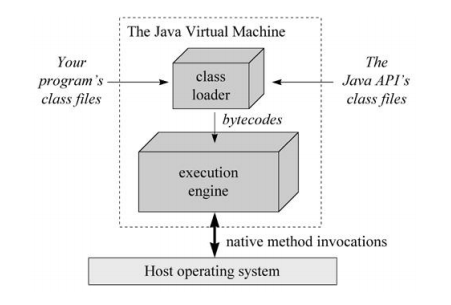
\includegraphics[scale=1]{imagens/jvm.png}
\end{figure}
 A \textbf{ Class loader} é a responsável por carregar os arquivos das classes do programa e da API
do Java, além de verificar a corretude das classes, inicializar a memória para as
variáveis de classe e ajudar na resolução de símbolos. [3]

\textbf{Execution engine} é onde os bytecodes são executados,e onde temos mais implementações
diferentes na JVM. [3]

\textbf{Native method invocations} é  o que faz a interação com o Sistema Operacional (SO),
onde se tem a ligação entre o JVM e o SO. Os métodos nativos geralmente são
escritos em C e C++. [3]

\section{Tipos de Dados do JVM}
No JVM existem tipos primitivos de dados, tais como byte, short, int, long, float, double e
referencias a objetos, etc... O tamanho de uma palavra(“word”) no JVM vária de acordo com a
implementação e deve ser grande o suficiente para armazenar os tipos primitivos supracitados, em
exceção ao long e double, que por sua vez duas words devem ser capazes de armazená-los.
Os tipos numéricos são subdivididos em tipos inteiros e em pontos flutuantes, como pode ser
visto abaixo:[3]\\
• byte - 9 bits com sinal\\
• char - 16 bits sem sinal\\
• short - 16 bits com sinal\\
• int - 32 bits com sinal\\
• long - 64 bits com sinal\\
• float - 32 bits com sinal\\
• double - 64 bits com sinal\\
\section{Instruções da JVM}
Uma instrução da JVM consiste de um opcode de um byte e pode ter argumentos e dados
que serão usandos na operação. A opção de ter a instrução em apenas um byte permite maior
simplicidade e limita o número de instruções.
O opcode mnemônico na maioria das instruções representa o tipo sobre qual ela opera. Possui
uma letra para representar cada tipo:[3]
• i: para int;\\
• l: para long;\\
• s: para short;\\
• b: para byte;\\
• c: para char;\\
• f: para float;\\
• d: ara double;\\
• a: para uma referência;
\chapter{Jasmin}
Neste capítulo aprofundamos as características do Jasmin.
\section{O que é Jasmin?}
 Jasmin é um assembler para Java Virtual Machine(JVM).A função dele é converter códigos escritos seguindo uma sintaxe assembler - que utiliza o conjunto de instruções da JVM - em códigos binários de classes Java adequados para serem carregados por um sistema Java Runtime. Resumindo, o Jasmin recebe um arquivo .j e produz um arquivo .class .\\
Sempre que possivel, o Jasmin adota um mapeamento   \texttt{one-to-one} entre sua sintaxe e as convenções seguidas pelos arquivos de classe Java.Por exemplo,os nomes dos pacotes em Jasmin são delimitados com o caractere   "\texttt{/}"  (por exemplo," \texttt{java/lang/String}" usado pelo formato de arquivo da classe,em vez do caractere   "\texttt{.}" (  \texttt{"java.lang.String"} )  usado na linguagem Java.\\ Usando o Jasmin,é possível experimentar quase todos os recursos da JVM,incluindo métodos,campos,sub-rotinas, \texttt{exception handlers},etc.
\section{Como executar o Jasmin?}
O arquivo jasmin.jar é um arquivo JAR executável que executa o Jasmin. Por exemplo:
\begin{terminal}
>   java -jar jasmin.jar nomedoarquivodesaida.j 
\end{terminal}
O Jasmin analisa a diretriz .class contida no arquivo nomedoarquivodesaida.j  para decidir onde colocar o arquivo de classe de saída. Então, se nomedoarquivodesaida.j  começar com:     ".class pacoteexemplo/MinhaClasse"
então Jasmin colocará o arquivo de classe de saída "MinhaClasse.class" no subdiretório "pacoteexemplo" do diretório atual. Ele criará o diretório pacoteexemplo se ele não existir.
Podemos  usar a opção "-d" para dizer ao jasmin que coloque a saída em um diretório alternativo. Por exemplo,
\begin{terminal}
>   java -jar jasmin.jar -d / tmp nomedoarquivodesaida.j 
\end{terminal}
Dessa forma a saída será gerada em /tmp/pacoteexemplo/MinhaClasse.class.


\section{Assembly Jasmin}
Jasmin usa o padrão para a JVM mnemônico (parâmetros) opcodes como instrução de nomes.
Os arquivos para Jasmin começam com as informações sobre a classe a ser definida no arquivo
- como o nome de classe, o nome do arquivo fonte que originou a partir da classe,o nome da
superclasse, etc.
 \textit{.font/opcional .class .super}

 O método (função) começa com  \textit{ .method} e termina com   \textit{ .end
method}. No método principal utiliza-se \textit{ .limit stack 5}
 (configura o tamanho da pilha para o método
principal (main) operando a 5) e  \textit{ .limit locals 100}
 (define o número de variáveis locais do método
principal (main) para 100).
Abaixo estão relatadas mais algumas instruções utilizadas no Jasmin:[3]\\ \\
 \textbf{iload} carrega o valor de uma variável local que é um inteiro para o topo da pilha.\\
 \textbf{istore} carrega o valor do topo da pilha para a variável.\\
 \textbf{fload} carrega o valor de uma variável local que é um float para o topo da pilha.\\
 \textbf{fstore} carrega o valor do topo da pilha que é um float para a variável.\\
 \textbf{ldc} desempilha a constante da pilha.\\
 \textbf{dup} a palavra no topo da pilha é duplicado.\\
 \textbf{pop} retira o valor que esta no topo da pilha.\\
 \textbf{swap} troca dois operandos da pilha (uma troca, o primeiro vira o segundo e o segundo vira o primeiro).\\
 \textbf{iadd} adiciona dois inteiros.\\
 \textbf{idiv} divide dois inteiros.\\
 \textbf{imul}  multiplica dois inteiros.\\
 \textbf{isub} subtrai dois inteiros.\\
 \textbf{fadd} adiciona dois float.\\
 \textbf{fdiv} divide dois float.\\
 \textbf{fmul} multiplica dois float.\\
 \textbf{fsub} subtrai dois float.\\
 \textbf{goto}  ir para o marcador.\\
 \textbf{ifeq} ir para o rótulo (marcador), se o valor no topo da pilha é 0.\\
 \textbf{ifge} ir para o rótulo, se o valor no topo da pilha é igual ou superior (maior) a 0.\\
 \textbf{ifgt} ir para o rótulo, se o valor no topo da pilha é superior (maior) a 0.\\
 \textbf{ifle} ir para o rótulo, se o valor no topo da pilha é inferior (menor) ou igual a 0.\\
 \textbf{iflt}ir para o rótulo, se o valor no topo da pilha é inferior (menor) a 0.\\
 \textbf{ifne} ir para o rótulo, se o valor no topo da pilha não é igual a 0.\\
 \textbf{iand} AND (inteiros).\\
 \textbf{ior } OR (inteiros).\\
 \textbf{ i2f} converte inteiro para float.\\
 \textbf{ f2i} converte float para inteiro.\\
 \textbf{ jsr} retorna o endereço da pilha e "pula"para subrotina indicada.\\
 \textbf{ ret} retorna o endereço da subrotina que esta armazenado a variável local.\\
 \textbf{ invokevirtual} é a forma padrão para a chamada de um método.\\ \\
Existem várias outras instruções como exemplo de mais algumas são: bipush, sipush, iinc, ifnull,
anewarray, checkcast, instanceof, new, getfeld, getstatic, putfeld, putstatic, newarray, iconst, entre outros.\\

\chapter{Exemplos de programas escritos em Java \label{ap:Testes}}
\section{Conversão para JAVA}
Todos os códigos Java foram gerados pelo javac com o seguinte  comando: 
\begin{terminal}
> javac nome.java
\end{terminal}


\section{Nano1.java}
\lstinputlisting[label={arq:Nano1.java}, language=Java,
caption={Nano1.java}]{codigos/MiniJava/Nano1.java}
\section{Nano2.java}
\lstinputlisting[label={arq:Nano2.java}, language=Java,
caption={Nano2.java}]{codigos/MiniJava/Nano2.java}
\section{Nano3.java}
\lstinputlisting[label={arq:Nano3.java}, language=Java,
caption={Nano3.java}]{codigos/MiniJava/Nano3.java}
\section{Nano4.java}
\lstinputlisting[label={arq:Nano4.java}, language=Java,
caption={Nano4.java}]{codigos/MiniJava/Nano4.java}
\section{Nano5.java}
\lstinputlisting[label={arq:Nano5.java}, language=Java,
caption={Nano5.java}]{codigos/MiniJava/Nano5.java}
\section{Nano6.java}
\lstinputlisting[label={arq:Nano6.java}, language=Java,
caption={Nano6.java}]{codigos/MiniJava/Nano6.java}
\section{Nano7.java}
\lstinputlisting[label={arq:Nano7.java}, language=Java,
caption={Nano7.java}]{codigos/MiniJava/Nano7.java}
\section{Nano8.java}
\lstinputlisting[label={arq:Nano8.java}, language=Java,
caption={Nano8.java}]{codigos/MiniJava/Nano8.java}
\section{Nano9.java}
\lstinputlisting[label={arq:Nano9.java}, language=Java,
caption={Nano9.java}]{codigos/MiniJava/Nano9.java}
\section{Nano10.java}
\lstinputlisting[label={arq:Nano10.java}, language=Java,
caption={Nano10.java}]{codigos/MiniJava/Nano10.java}
\section{Nano11.java}
\lstinputlisting[label={arq:Nano11.java}, language=Java,
caption={Nano11.java}]{codigos/MiniJava/Nano11.java}
\section{Nano12.java}
\lstinputlisting[label={arq:Nano12.java}, language=Java,
caption={Nano12.java}]{codigos/MiniJava/Nano12.java}

\section{Micro1.java}
\lstinputlisting[label={arq:Micro1.java}, language=Java,
caption={Micro1.java}]{codigos/MiniJava/Micro1.java}
\section{Micro2.java}
\lstinputlisting[label={arq:Micro2.java}, language=Java,
caption={Micro2.java}]{codigos/MiniJava/Micro2.java}
\section{Micro3.java}
\lstinputlisting[label={arq:Micro3.java}, language=Java,
caption={Micro3.java}]{codigos/MiniJava/Micro3.java}
\section{Micro4.java}
\lstinputlisting[label={arq:Micro4.java}, language=Java,
caption={Micro4.java}]{codigos/MiniJava/Micro4.java}
\section{Micro5.java}
\lstinputlisting[label={arq:Micro5.java}, language=Java,
caption={Micro5.java}]{codigos/MiniJava/Micro5.java}
\section{Micro6.java}
\lstinputlisting[label={arq:Micro6.java}, language=Java,
caption={Micro6.java}]{codigos/MiniJava/Micro6.java}
\section{Micro7.java}
\lstinputlisting[label={arq:Micro7.java}, language=Java,
caption={Micro7.java}]{codigos/MiniJava/Micro7.java}
\section{Micro8.java}
\lstinputlisting[label={arq:Micro8.java}, language=Java,
caption={Micro8.java}]{codigos/MiniJava/Micro8.java}
\section{Micro9.java}
\lstinputlisting[label={arq:Micro9.java}, language=Java,
caption={Micro9.java}]{codigos/MiniJava/Micro9.java}
\section{Micro10.java}
\lstinputlisting[label={arq:Micro10.java}, language=Java,
caption={Micro10.java}]{codigos/MiniJava/Micro10.java}
\section{Micro11.java}
\lstinputlisting[label={arq:Micro11.java}, language=Java,
caption={Micro11.java}]{codigos/MiniJava/Micro11.java}


\chapter{Exemplos de programas escritos em Java convertidos para Assembly \label{ap:Testes}}
\section{Conversão para Assembly}
Todos os codigos Java para Assembly foram convertidos usando o comando javap da seguinte forma:
\begin{terminal}
javap -c nome.class
\end{terminal} 
Depois disso modificamos a saída desse comando para um arquivo Jasmin válido (um arquivo .j) .
\section{NanoPrograma1}
\begin{terminal}
.class public Nano1
.super java/lang/Object

.method public <init>()V
  .limit stack 1
  .limit locals 1
  .line 2
  0: aload_0
  1: invokespecial java/lang/Object/<init>()V
  4: return
.end method

.method public static main([Ljava/lang/String;)V
  .limit stack 0
  .limit locals 1
  .line 4
  0: return
.end method

\end{terminal}

\section{NanoPrograma2}
\begin{terminal}
.class public Nano2
.super java/lang/Object

.method public <init>()V
  .limit stack 1
  .limit locals 1
  .line 3
  0: aload_0
  1: invokespecial java/lang/Object/<init>()V
  4: return
.end method

.method public static main([Ljava/lang/String;)V
  .limit stack 0
  .limit locals 2
  .line 6
  0: return
.end method

\end{terminal}\section{NanoPrograma3}
\begin{terminal}
.class public Nano3
.super java/lang/Object

.method public <init>()V
  .limit stack 1
  .limit locals 1
  .line 3
  0: aload_0
  1: invokespecial java/lang/Object/<init>()V
  4: return
.end method

.method public static main([Ljava/lang/String;)V
  .limit stack 1
  .limit locals 2
  .line 6
  0: iconst_1
  1: istore_1
  .line 7
  2: return
.end method
\end{terminal}\section{NanoPrograma4}
\begin{terminal}
.class public Nano4
.super java/lang/Object

.method public <init>()V
  .limit stack 1
  .limit locals 1
  .line 3
  0: aload_0
  1: invokespecial java/lang/Object/<init>()V
  4: return
.end method

.method public static main([Ljava/lang/String;)V
  .limit stack 1
  .limit locals 2
  .line 6
  0: iconst_3
  1: istore_1
  .line 7
  2: return
.end method
\end{terminal}\section{NanoPrograma5}
\begin{terminal}
.class public Nano5
.super java/lang/Object

.method public <init>()V
  .limit stack 1
  .limit locals 1
  .line 3
  0: aload_0
  1: invokespecial java/lang/Object/<init>()V
  4: return
.end method

.method public static main([Ljava/lang/String;)V
  .limit stack 2
  .limit locals 2
  .line 6
  0: iconst_2
  1: istore_1
  .line 7
  2: getstatic java/lang/System/out Ljava/io/PrintStream;
  5: iload_1
  6: invokevirtual java/io/PrintStream/print(I)V
  .line 8
  9: return
.end method

\end{terminal}\section{NanoPrograma6}
\begin{terminal}
.class public Nano6
.super java/lang/Object

.method public <init>()V
  .limit stack 1
  .limit locals 1
  .line 3
  0: aload_0
  1: invokespecial java/lang/Object/<init>()V
  4: return
.end method

.method public static main([Ljava/lang/String;)V
  .limit stack 2
  .limit locals 2
  .line 6
  0: iconst_m1
  1: istore_1
  .line 7
  2: getstatic java/lang/System/out Ljava/io/PrintStream;
  5: iload_1
  6: invokevirtual java/io/PrintStream/print(I)V
  .line 9
  9: return
.end method
\end{terminal}\section{NanoPrograma7}
\begin{terminal}
.class public Nano7
.super java/lang/Object

.method public <init>()V
  .limit stack 1
  .limit locals 1
  .line 3
  0: aload_0
  1: invokespecial java/lang/Object/<init>()V
  4: return
.end method

.method public static main([Ljava/lang/String;)V
  .limit stack 2
  .limit locals 2
  .line 6
  0: iconst_1
  1: istore_1
  .line 7
  2: iload_1
  3: iconst_1
  4: if_icmpne Label14
  .line 8
  7: getstatic java/lang/System/out Ljava/io/PrintStream;
  10: iload_1
  11: invokevirtual java/io/PrintStream/print(I)V
Label14:
  .line 10
  14: return
  ; append_frame (frameNumber = 0)
  ; frame_type = 252, offset_delta = 14
  ; frame bytes: 252 0 14 1
  .stack
    offset 14
    locals Integer
    .end stack
.end method

\end{terminal}\section{NanoPrograma8}
\begin{terminal}
.class public Nano8
.super java/lang/Object

.method public <init>()V
  .limit stack 1
  .limit locals 1
  .line 3
  0: aload_0
  1: invokespecial java/lang/Object/<init>()V
  4: return
.end method

.method public static main([Ljava/lang/String;)V
  .limit stack 2
  .limit locals 2
  .line 6
  0: iconst_1
  1: istore_1
  .line 7
  2: iload_1
  3: iconst_1
  4: if_icmpne Label17
  .line 8
  7: getstatic java/lang/System/out Ljava/io/PrintStream;
  10: iload_1
  11: invokevirtual java/io/PrintStream/print(I)V
  14: goto Label25
Label17:
  .line 11
  17: getstatic java/lang/System/out Ljava/io/PrintStream;
  20: ldc "0"
  22: invokevirtual java/io/PrintStream/print(Ljava/lang/String;)V
Label25:
  .line 14
  25: return
  ; append_frame (frameNumber = 0)
  ; frame_type = 252, offset_delta = 17
  ; frame bytes: 252 0 17 1
  .stack
    offset 17
    locals Integer
    .end stack
  ; same_frame (frameNumber = 1)
  ; frame_type = 7, offset_delta = 7
  ; frame bytes: 7
  .stack
    offset 25
    locals Integer
    .end stack
.end method
\end{terminal}\section{NanoPrograma9}
\begin{terminal}
.class public Nano9
.super java/lang/Object

.method public <init>()V
  .limit stack 1
  .limit locals 1
  .line 3
  0: aload_0
  1: invokespecial java/lang/Object/<init>()V
  4: return
.end method

.method public static main([Ljava/lang/String;)V
  .limit stack 2
  .limit locals 2
  .line 6
  0: iconst_1
  1: istore_1
  .line 7
  2: iload_1
  3: iconst_1
  4: if_icmpne Label17
  .line 8
  7: getstatic java/lang/System/out Ljava/io/PrintStream;
  10: iload_1
  11: invokevirtual java/io/PrintStream/print(I)V
  14: goto Label25
Label17:
  .line 10
  17: getstatic java/lang/System/out Ljava/io/PrintStream;
  20: ldc "0"
  22: invokevirtual java/io/PrintStream/print(Ljava/lang/String;)V
Label25:
  .line 13
  25: return
  ; append_frame (frameNumber = 0)
  ; frame_type = 252, offset_delta = 17
  ; frame bytes: 252 0 17 1
  .stack
    offset 17
    locals Integer
    .end stack
  ; same_frame (frameNumber = 1)
  ; frame_type = 7, offset_delta = 7
  ; frame bytes: 7
  .stack
    offset 25
    locals Integer
    .end stack
.end method
\end{terminal}\section{NanoPrograma10}
\begin{terminal}
.class public Nano10
.super java/lang/Object

.method public <init>()V
  .limit stack 1
  .limit locals 1
  .line 3
  0: aload_0
  1: invokespecial java/lang/Object/<init>()V
  4: return
.end method

.method public static main([Ljava/lang/String;)V
  .limit stack 2
  .limit locals 3
  .line 6
  0: iconst_1
  1: istore_1
  .line 7
  2: iconst_2
  3: istore_2
  .line 8
  4: iload_1
  5: iload_2
  6: if_icmpne Label19
  .line 9
  9: getstatic java/lang/System/out Ljava/io/PrintStream;
  12: iload_1
  13: invokevirtual java/io/PrintStream/print(I)V
  16: goto Label27
Label19:
  .line 11
  19: getstatic java/lang/System/out Ljava/io/PrintStream;
  22: ldc "0"
  24: invokevirtual java/io/PrintStream/print(Ljava/lang/String;)V
Label27:
  .line 14
  27: return
  ; append_frame (frameNumber = 0)
  ; frame_type = 253, offset_delta = 19
  ; frame bytes: 253 0 19 1 1
  .stack
    offset 19
    locals Integer
    locals Integer
    .end stack
  ; same_frame (frameNumber = 1)
  ; frame_type = 7, offset_delta = 7
  ; frame bytes: 7
  .stack
    offset 27
    locals Integer
    locals Integer
    .end stack
.end method
\end{terminal}\section{NanoPrograma11}
\begin{terminal}
.class public Nano11
.super java/lang/Object

.method public <init>()V
  .limit stack 1
  .limit locals 1
  .line 2
  0: aload_0
  1: invokespecial java/lang/Object/<init>()V
  4: return
.end method

.method public static main([Ljava/lang/String;)V
  .limit stack 2
  .limit locals 4
  .line 5
  0: iconst_1
  1: istore_1
  .line 6
  2: iconst_2
  3: istore_2
  .line 7
  4: iconst_5
  5: istore_3
Label6:
  .line 8
  6: iload_3
  7: iload_1
  8: if_icmple Label18
  .line 9
  11: iload_1
  12: iload_2
  13: iadd
  14: istore_1
  15: goto Label6
Label18:
  .line 11
  18: return
  ; append_frame (frameNumber = 0)
  ; frame_type = 254, offset_delta = 6
  ; frame bytes: 254 0 6 1 1 1
  .stack
    offset 6
    locals Integer
    locals Integer
    locals Integer
    .end stack
  ; same_frame (frameNumber = 1)
  ; frame_type = 11, offset_delta = 11
  ; frame bytes: 11
  .stack
    offset 18
    locals Integer
    locals Integer
    locals Integer
    .end stack
.end method
\end{terminal}\section{NanoPrograma12}
\begin{terminal}
.class public Nano12
.super java/lang/Object

.method public <init>()V
  .limit stack 1
  .limit locals 1
  .line 3
  0: aload_0
  1: invokespecial java/lang/Object/<init>()V
  4: return
.end method

.method public static main([Ljava/lang/String;)V
  .limit stack 2
  .limit locals 4
  .line 6
  0: iconst_1
  1: istore_1
  .line 7
  2: iconst_2
  3: istore_2
  .line 8
  4: iconst_5
  5: istore_3
Label6:
  .line 9
  6: iload_3
  7: iload_1
  8: if_icmple Label40
  .line 10
  11: iload_1
  12: iload_2
  13: if_icmpne Label26
  .line 11
  16: getstatic java/lang/System/out Ljava/io/PrintStream;
  19: iload_1
  20: invokevirtual java/io/PrintStream/print(I)V
  23: goto Label33
Label26:
  .line 13
  26: getstatic java/lang/System/out Ljava/io/PrintStream;
  29: iconst_0
  30: invokevirtual java/io/PrintStream/print(I)V
Label33:
  .line 15
  33: iload_3
  34: iconst_1
  35: isub
  36: istore_3
  37: goto Label6
Label40:
  .line 17
  40: return
  ; append_frame (frameNumber = 0)
  ; frame_type = 254, offset_delta = 6
  ; frame bytes: 254 0 6 1 1 1
  .stack
    offset 6
    locals Integer
    locals Integer
    locals Integer
    .end stack
  ; same_frame (frameNumber = 1)
  ; frame_type = 19, offset_delta = 19
  ; frame bytes: 19
  .stack
    offset 26
    locals Integer
    locals Integer
    locals Integer
    .end stack
  ; same_frame (frameNumber = 2)
  ; frame_type = 6, offset_delta = 6
  ; frame bytes: 6
  .stack
    offset 33
    locals Integer
    locals Integer
    locals Integer
    .end stack
  ; same_frame (frameNumber = 3)
  ; frame_type = 6, offset_delta = 6
  ; frame bytes: 6
  .stack
    offset 40
    locals Integer
    locals Integer
    locals Integer
    .end stack
.end method

\end{terminal}

\section{MicroPrograma1}
\begin{terminal}
.class public Micro1
.super java/lang/Object

.method public <init>()V
  .limit stack 1
  .limit locals 1
  .line 3
  0: aload_0
  1: invokespecial java/lang/Object/<init>()V
  4: return
.end method

.method public static main([Ljava/lang/String;)V
  .limit stack 4
  .limit locals 6
  .line 6
  0: getstatic java/lang/System/out Ljava/io/PrintStream;
  3: ldc "Tabela de conversao: Celsius -> Fahrenheit"
  5: invokevirtual java/io/PrintStream/println(Ljava/lang/String;)V
  .line 7
  8: getstatic java/lang/System/out Ljava/io/PrintStream;
  11: ldc "Digite a temperatura em Celsius:"
  13: invokevirtual java/io/PrintStream/println(Ljava/lang/String;)V
  .line 8
  16: new java/util/Scanner
  19: dup
  20: getstatic java/lang/System/in Ljava/io/InputStream;
  23: invokespecial java/util/Scanner/<init>(Ljava/io/InputStream;)V
  26: astore 5
  .line 9
  28: aload 5
  30: invokevirtual java/util/Scanner/nextDouble()D
  33: dstore_1
  .line 10
  34: ldc2_w 9.0
  37: dload_1
  38: dmul
  39: ldc2_w 160.0
  42: dadd
  43: ldc2_w 5.0
  46: ddiv
  47: dstore_3
  .line 11
  48: getstatic java/lang/System/out Ljava/io/PrintStream;
  51: new java/lang/StringBuilder
  54: dup
  55: invokespecial java/lang/StringBuilder/<init>()V
  58: ldc "A nova temperatura eh "
  60: invokevirtual java/lang/StringBuilder/append(Ljava/lang/String;)Ljava/lang/StringBuilder;
  63: dload_3
  64: invokevirtual java/lang/StringBuilder/append(D)Ljava/lang/StringBuilder;
  67: ldc " F"
  69: invokevirtual java/lang/StringBuilder/append(Ljava/lang/String;)Ljava/lang/StringBuilder;
  72: invokevirtual java/lang/StringBuilder/toString()Ljava/lang/String;
  75: invokevirtual java/io/PrintStream/println(Ljava/lang/String;)V
  .line 12
  78: return
.end method
\end{terminal}


\section{MicroPrograma2}
\begin{terminal}

.class public Micro2
.super java/lang/Object

.method public <init>()V
  .limit stack 1
  .limit locals 1
  .line 3
  0: aload_0
  1: invokespecial java/lang/Object/<init>()V
  4: return
.end method

.method public static main([Ljava/lang/String;)V
  .limit stack 3
  .limit locals 4
  .line 6
  0: new java/util/Scanner
  3: dup
  4: getstatic java/lang/System/in Ljava/io/InputStream;
  7: invokespecial java/util/Scanner/<init>(Ljava/io/InputStream;)V
  10: astore_3
  .line 7
  11: getstatic java/lang/System/out Ljava/io/PrintStream;
  14: ldc "Digite o primeiro numero: "
  16: invokevirtual java/io/PrintStream/println(Ljava/lang/String;)V
  .line 8
  19: aload_3
  20: invokevirtual java/util/Scanner/nextInt()I
  23: istore_1
  .line 9
  24: getstatic java/lang/System/out Ljava/io/PrintStream;
  27: ldc "Digite o segundo numero:"
  29: invokevirtual java/io/PrintStream/println(Ljava/lang/String;)V
  .line 10
  32: aload_3
  33: invokevirtual java/util/Scanner/nextInt()I
  36: istore_2
  .line 11
  37: iload_1
  38: iload_2
  39: if_icmple Label79
  .line 12
  42: getstatic java/lang/System/out Ljava/io/PrintStream;
  45: new java/lang/StringBuilder
  48: dup
  49: invokespecial java/lang/StringBuilder/<init>()V
  52: ldc "O primeiro numero "
  54: invokevirtual java/lang/StringBuilder/append(Ljava/lang/String;)Ljava/lang/StringBuilder;
  57: iload_1
  58: invokevirtual java/lang/StringBuilder/append(I)Ljava/lang/StringBuilder;
  61: ldc " eh maior que o segundo "
  63: invokevirtual java/lang/StringBuilder/append(Ljava/lang/String;)Ljava/lang/StringBuilder;
  66: iload_2
  67: invokevirtual java/lang/StringBuilder/append(I)Ljava/lang/StringBuilder;
  70: invokevirtual java/lang/StringBuilder/toString()Ljava/lang/String;
  73: invokevirtual java/io/PrintStream/println(Ljava/lang/String;)V
  76: goto Label113
Label79:
  .line 14
  79: getstatic java/lang/System/out Ljava/io/PrintStream;
  82: new java/lang/StringBuilder
  85: dup
  86: invokespecial java/lang/StringBuilder/<init>()V
  89: ldc "O segundo numero "
  91: invokevirtual java/lang/StringBuilder/append(Ljava/lang/String;)Ljava/lang/StringBuilder;
  94: iload_2
  95: invokevirtual java/lang/StringBuilder/append(I)Ljava/lang/StringBuilder;
  98: ldc " eh maior que o primeiro"
  100: invokevirtual java/lang/StringBuilder/append(Ljava/lang/String;)Ljava/lang/StringBuilder;
  103: iload_2
  104: invokevirtual java/lang/StringBuilder/append(I)Ljava/lang/StringBuilder;
  107: invokevirtual java/lang/StringBuilder/toString()Ljava/lang/String;
  110: invokevirtual java/io/PrintStream/println(Ljava/lang/String;)V
Label113:
  .line 16
  113: return
  ; append_frame (frameNumber = 0)
  ; frame_type = 254, offset_delta = 79
  ; frame bytes: 254 0 79 1 1 7 0 28
  .stack
    offset 79
    locals Integer
    locals Integer
    locals Object java/util/Scanner
    .end stack
  ; same_frame (frameNumber = 1)
  ; frame_type = 33, offset_delta = 33
  ; frame bytes: 33
  .stack
    offset 113
    locals Integer
    locals Integer
    locals Object java/util/Scanner
    .end stack
.end method
\end{terminal}


\section{MicroPrograma3}
\begin{terminal}
.class public Micro3
.super java/lang/Object

.method public <init>()V
  .limit stack 1
  .limit locals 1
  .line 3
  0: aload_0
  1: invokespecial java/lang/Object/<init>()V
  4: return
.end method

.method public static main([Ljava/lang/String;)V
  .limit stack 3
  .limit locals 3
  .line 6
  0: getstatic java/lang/System/out Ljava/io/PrintStream;
  3: ldc "Digite o numero: "
  5: invokevirtual java/io/PrintStream/println(Ljava/lang/String;)V
  .line 7
  8: new java/util/Scanner
  11: dup
  12: getstatic java/lang/System/in Ljava/io/InputStream;
  15: invokespecial java/util/Scanner/<init>(Ljava/io/InputStream;)V
  18: astore_2
  .line 8
  19: aload_2
  20: invokevirtual java/util/Scanner/nextInt()I
  23: istore_1
  .line 9
  24: iload_1
  25: bipush 100
  27: if_icmplt Label59
  .line 10
  30: iload_1
  31: sipush 200
  34: if_icmpgt Label48
  .line 11
  37: getstatic java/lang/System/out Ljava/io/PrintStream;
  40: ldc "O numero esta no intervalo entre 100 e 200"
  42: invokevirtual java/io/PrintStream/println(Ljava/lang/String;)V
  45: goto Label67
Label48:
  .line 14
  48: getstatic java/lang/System/out Ljava/io/PrintStream;
  51: ldc "O numero nao esta no intervalo entre 100 e 200"
  53: invokevirtual java/io/PrintStream/println(Ljava/lang/String;)V
  56: goto Label67
Label59:
  .line 18
  59: getstatic java/lang/System/out Ljava/io/PrintStream;
  62: ldc "O numero nao esta no intervalo entre 100 e 200"
  64: invokevirtual java/io/PrintStream/println(Ljava/lang/String;)V
Label67:
  .line 20
  67: return
  ; append_frame (frameNumber = 0)
  ; frame_type = 253, offset_delta = 48
  ; frame bytes: 253 0 48 1 7 0 20
  .stack
    offset 48
    locals Integer
    locals Object java/util/Scanner
    .end stack
  ; same_frame (frameNumber = 1)
  ; frame_type = 10, offset_delta = 10
  ; frame bytes: 10
  .stack
    offset 59
    locals Integer
    locals Object java/util/Scanner
    .end stack
  ; same_frame (frameNumber = 2)
  ; frame_type = 7, offset_delta = 7
  ; frame bytes: 7
  .stack
    offset 67
    locals Integer
    locals Object java/util/Scanner
    .end stack
.end method

\end{terminal}


\section{MicroPrograma4}
\begin{terminal}
.class public Micro4
.super java/lang/Object

.method public <init>()V
  .limit stack 1
  .limit locals 1
  .line 3
  0: aload_0
  1: invokespecial java/lang/Object/<init>()V
  4: return
.end method

.method public static main([Ljava/lang/String;)V
  .limit stack 3
  .limit locals 5
  .line 6
  0: iconst_0
  1: istore_3
  .line 7
  2: iconst_1
  3: istore_1
Label4:
  4: iload_1
  5: iconst_5
  6: if_icmpgt Label58
  .line 8
  9: getstatic java/lang/System/out Ljava/io/PrintStream;
  12: ldc "Digite o numero: "
  14: invokevirtual java/io/PrintStream/println(Ljava/lang/String;)V
  .line 9
  17: new java/util/Scanner
  20: dup
  21: getstatic java/lang/System/in Ljava/io/InputStream;
  24: invokespecial java/util/Scanner/<init>(Ljava/io/InputStream;)V
  27: astore 4
  .line 10
  29: aload 4
  31: invokevirtual java/util/Scanner/nextInt()I
  34: istore_2
  .line 11
  35: iload_2
  36: bipush 10
  38: if_icmplt Label52
  .line 12
  41: iload_2
  42: sipush 150
  45: if_icmpgt Label52
  .line 13
  48: iload_3
  49: iconst_1
  50: iadd
  51: istore_3
Label52:
  .line 7
  52: iinc 1 1
  55: goto Label4
Label58:
  .line 16
  58: getstatic java/lang/System/out Ljava/io/PrintStream;
  61: new java/lang/StringBuilder
  64: dup
  65: invokespecial java/lang/StringBuilder/<init>()V
  68: ldc "Ao total, foram digitados "
  70: invokevirtual java/lang/StringBuilder/append(Ljava/lang/String;)Ljava/lang/StringBuilder;
  73: iload_3
  74: invokevirtual java/lang/StringBuilder/append(I)Ljava/lang/StringBuilder;
  77: ldc " numeros no intervalo entre 10 e 150"
  79: invokevirtual java/lang/StringBuilder/append(Ljava/lang/String;)Ljava/lang/StringBuilder;
  82: invokevirtual java/lang/StringBuilder/toString()Ljava/lang/String;
  85: invokevirtual java/io/PrintStream/println(Ljava/lang/String;)V
  .line 18
  88: return
  ; append_frame (frameNumber = 0)
  ; frame_type = 254, offset_delta = 4
  ; frame bytes: 254 0 4 1 0 1
  .stack
    offset 4
    locals Integer
    locals Top
    locals Integer
    .end stack
  ; full_frame (frameNumber = 1)
  ; frame_type = 255, offset_delta = 47
  ; frame bytes: 255 0 47 0 4 7 0 25 1 1 1 0 0
  .stack
    offset 52
    locals Object [Ljava/lang/String;
    locals Integer
    locals Integer
    locals Integer
    .end stack
  ; full_frame (frameNumber = 2)
  ; frame_type = 255, offset_delta = 5
  ; frame bytes: 255 0 5 0 4 7 0 25 1 0 1 0 0
  .stack
    offset 58
    locals Object [Ljava/lang/String;
    locals Integer
    locals Top
    locals Integer
    .end stack
.end method

\end{terminal}


\section{MicroPrograma5}
\begin{terminal}
.class public Micro5
.super java/lang/Object

.method public <init>()V
  .limit stack 1
  .limit locals 1
  .line 3
  0: aload_0
  1: invokespecial java/lang/Object/<init>()V
  4: return
.end method

.method public static main([Ljava/lang/String;)V
  .limit stack 3
  .limit locals 7
  .line 6
  0: new java/util/Scanner
  3: dup
  4: getstatic java/lang/System/in Ljava/io/InputStream;
  7: invokespecial java/util/Scanner/<init>(Ljava/io/InputStream;)V
  10: astore_2
  .line 9
  11: iconst_0
  12: istore 5
  .line 10
  14: iconst_0
  15: istore 6
  .line 11
  17: iconst_0
  18: istore 6
  .line 12
  20: iconst_1
  21: istore 4
Label23:
  23: iload 4
  25: iconst_5
  26: if_icmpgt Label120
  .line 13
  29: getstatic java/lang/System/out Ljava/io/PrintStream;
  32: ldc "Digite o nome: "
  34: invokevirtual java/io/PrintStream/println(Ljava/lang/String;)V
  .line 14
  37: aload_2
  38: invokevirtual java/util/Scanner/nextLine()Ljava/lang/String;
  41: astore_1
  .line 15
  42: getstatic java/lang/System/out Ljava/io/PrintStream;
  45: ldc "Digite o sexo: "
  47: invokevirtual java/io/PrintStream/println(Ljava/lang/String;)V
  .line 16
  50: aload_2
  51: invokevirtual java/util/Scanner/nextLine()Ljava/lang/String;
  54: iconst_0
  55: invokevirtual java/lang/String/charAt(I)C
  58: istore_3
  .line 17
  59: iload_3
  60: lookupswitch
          72 : Label88
          77 : Label97
          default : Label106
Label88:
  .line 18
  88: iload 5
  90: iconst_1
  91: iadd
  92: istore 5
  94: goto Label114
Label97:
  .line 19
  97: iload 6
  99: iconst_1
  100: iadd
  101: istore 6
  103: goto Label114
Label106:
  .line 20
  106: getstatic java/lang/System/out Ljava/io/PrintStream;
  109: ldc "Atencao sexo pode ser H ou M!"
  111: invokevirtual java/io/PrintStream/println(Ljava/lang/String;)V
Label114:
  .line 12
  114: iinc 4 1
  117: goto Label23
Label120:
  .line 24
  120: getstatic java/lang/System/out Ljava/io/PrintStream;
  123: new java/lang/StringBuilder
  126: dup
  127: invokespecial java/lang/StringBuilder/<init>()V
  130: ldc "Foram inseridos "
  132: invokevirtual java/lang/StringBuilder/append(Ljava/lang/String;)Ljava/lang/StringBuilder;
  135: iload 5
  137: invokevirtual java/lang/StringBuilder/append(I)Ljava/lang/StringBuilder;
  140: ldc " Homens"
  142: invokevirtual java/lang/StringBuilder/append(Ljava/lang/String;)Ljava/lang/StringBuilder;
  145: invokevirtual java/lang/StringBuilder/toString()Ljava/lang/String;
  148: invokevirtual java/io/PrintStream/println(Ljava/lang/String;)V
  .line 25
  151: getstatic java/lang/System/out Ljava/io/PrintStream;
  154: new java/lang/StringBuilder
  157: dup
  158: invokespecial java/lang/StringBuilder/<init>()V
  161: ldc "Foram inseridos "
  163: invokevirtual java/lang/StringBuilder/append(Ljava/lang/String;)Ljava/lang/StringBuilder;
  166: iload 6
  168: invokevirtual java/lang/StringBuilder/append(I)Ljava/lang/StringBuilder;
  171: ldc " Mulheres"
  173: invokevirtual java/lang/StringBuilder/append(Ljava/lang/String;)Ljava/lang/StringBuilder;
  176: invokevirtual java/lang/StringBuilder/toString()Ljava/lang/String;
  179: invokevirtual java/io/PrintStream/println(Ljava/lang/String;)V
  .line 26
  182: return
  ; full_frame (frameNumber = 0)
  ; frame_type = 255, offset_delta = 23
  ; frame bytes: 255 0 23 0 7 7 0 29 0 7 0 30 0 1 1 1 0 0
  .stack
    offset 23
    locals Object [Ljava/lang/String;
    locals Top
    locals Object java/util/Scanner
    locals Top
    locals Integer
    locals Integer
    locals Integer
    .end stack
  ; full_frame (frameNumber = 1)
  ; frame_type = 255, offset_delta = 64
  ; frame bytes: 255 0 64 0 7 7 0 29 7 0 31 7 0 30 1 1 1 1 0 0
  .stack
    offset 88
    locals Object [Ljava/lang/String;
    locals Object java/lang/String
    locals Object java/util/Scanner
    locals Integer
    locals Integer
    locals Integer
    locals Integer
    .end stack
  ; same_frame (frameNumber = 2)
  ; frame_type = 8, offset_delta = 8
  ; frame bytes: 8
  .stack
    offset 97
    locals Object [Ljava/lang/String;
    locals Object java/lang/String
    locals Object java/util/Scanner
    locals Integer
    locals Integer
    locals Integer
    locals Integer
    .end stack
  ; same_frame (frameNumber = 3)
  ; frame_type = 8, offset_delta = 8
  ; frame bytes: 8
  .stack
    offset 106
    locals Object [Ljava/lang/String;
    locals Object java/lang/String
    locals Object java/util/Scanner
    locals Integer
    locals Integer
    locals Integer
    locals Integer
    .end stack
  ; same_frame (frameNumber = 4)
  ; frame_type = 7, offset_delta = 7
  ; frame bytes: 7
  .stack
    offset 114
    locals Object [Ljava/lang/String;
    locals Object java/lang/String
    locals Object java/util/Scanner
    locals Integer
    locals Integer
    locals Integer
    locals Integer
    .end stack
  ; full_frame (frameNumber = 5)
  ; frame_type = 255, offset_delta = 5
  ; frame bytes: 255 0 5 0 7 7 0 29 0 7 0 30 0 1 1 1 0 0
  .stack
    offset 120
    locals Object [Ljava/lang/String;
    locals Top
    locals Object java/util/Scanner
    locals Top
    locals Integer
    locals Integer
    locals Integer
    .end stack
.end method


\end{terminal}


\section{MicroPrograma6}
\begin{terminal}
.class public Micro6
.super java/lang/Object

.method public <init>()V
  .limit stack 1
  .limit locals 1
  .line 3
  0: aload_0
  1: invokespecial java/lang/Object/<init>()V
  4: return
.end method

.method public static main([Ljava/lang/String;)V
  .limit stack 3
  .limit locals 3
  .line 6
  0: getstatic java/lang/System/out Ljava/io/PrintStream;
  3: ldc "Digite um numero de 1 a 5: "
  5: invokevirtual java/io/PrintStream/println(Ljava/lang/String;)V
  .line 7
  8: new java/util/Scanner
  11: dup
  12: getstatic java/lang/System/in Ljava/io/InputStream;
  15: invokespecial java/util/Scanner/<init>(Ljava/io/InputStream;)V
  18: astore_2
  .line 8
  19: aload_2
  20: invokevirtual java/util/Scanner/nextInt()I
  23: istore_1
  .line 9
  24: iload_1
  25: tableswitch 1 5
          Label60
          Label71
          Label82
          Label93
          Label104
          default : Label115
Label60:
  .line 10
  60: getstatic java/lang/System/out Ljava/io/PrintStream;
  63: ldc "Um"
  65: invokevirtual java/io/PrintStream/println(Ljava/lang/String;)V
  68: goto Label123
Label71:
  .line 11
  71: getstatic java/lang/System/out Ljava/io/PrintStream;
  74: ldc "Dois"
  76: invokevirtual java/io/PrintStream/println(Ljava/lang/String;)V
  79: goto Label123
Label82:
  .line 12
  82: getstatic java/lang/System/out Ljava/io/PrintStream;
  85: ldc "Tres"
  87: invokevirtual java/io/PrintStream/println(Ljava/lang/String;)V
  90: goto Label123
Label93:
  .line 13
  93: getstatic java/lang/System/out Ljava/io/PrintStream;
  96: ldc "Quatro"
  98: invokevirtual java/io/PrintStream/println(Ljava/lang/String;)V
  101: goto Label123
Label104:
  .line 14
  104: getstatic java/lang/System/out Ljava/io/PrintStream;
  107: ldc "Cinco"
  109: invokevirtual java/io/PrintStream/println(Ljava/lang/String;)V
  112: goto Label123
Label115:
  .line 15
  115: getstatic java/lang/System/out Ljava/io/PrintStream;
  118: ldc "numero invalido!!!"
  120: invokevirtual java/io/PrintStream/println(Ljava/lang/String;)V
Label123:
  .line 17
  123: return
  ; append_frame (frameNumber = 0)
  ; frame_type = 253, offset_delta = 60
  ; frame bytes: 253 0 60 1 7 0 24
  .stack
    offset 60
    locals Integer
    locals Object java/util/Scanner
    .end stack
  ; same_frame (frameNumber = 1)
  ; frame_type = 10, offset_delta = 10
  ; frame bytes: 10
  .stack
    offset 71
    locals Integer
    locals Object java/util/Scanner
    .end stack
  ; same_frame (frameNumber = 2)
  ; frame_type = 10, offset_delta = 10
  ; frame bytes: 10
  .stack
    offset 82
    locals Integer
    locals Object java/util/Scanner
    .end stack
  ; same_frame (frameNumber = 3)
  ; frame_type = 10, offset_delta = 10
  ; frame bytes: 10
  .stack
    offset 93
    locals Integer
    locals Object java/util/Scanner
    .end stack
  ; same_frame (frameNumber = 4)
  ; frame_type = 10, offset_delta = 10
  ; frame bytes: 10
  .stack
    offset 104
    locals Integer
    locals Object java/util/Scanner
    .end stack
  ; same_frame (frameNumber = 5)
  ; frame_type = 10, offset_delta = 10
  ; frame bytes: 10
  .stack
    offset 115
    locals Integer
    locals Object java/util/Scanner
    .end stack
  ; same_frame (frameNumber = 6)
  ; frame_type = 7, offset_delta = 7
  ; frame bytes: 7
  .stack
    offset 123
    locals Integer
    locals Object java/util/Scanner
    .end stack
.end method

\end{terminal}


\section{MicroPrograma7}
\begin{terminal}
.class public Micro7
.super java/lang/Object

.method public <init>()V
  .limit stack 1
  .limit locals 1
  .line 3
  0: aload_0
  1: invokespecial java/lang/Object/<init>()V
  4: return
.end method

.method public static main([Ljava/lang/String;)V
  .limit stack 3
  .limit locals 5
  .line 7
  0: iconst_1
  1: istore_1
Label2:
  .line 8
  2: iload_1
  3: iconst_1
  4: if_icmpne Label101
  .line 9
  7: getstatic java/lang/System/out Ljava/io/PrintStream;
  10: ldc "Digite um numero: "
  12: invokevirtual java/io/PrintStream/println(Ljava/lang/String;)V
  .line 10
  15: new java/util/Scanner
  18: dup
  19: getstatic java/lang/System/in Ljava/io/InputStream;
  22: invokespecial java/util/Scanner/<init>(Ljava/io/InputStream;)V
  25: astore 4
  .line 11
  27: aload 4
  29: invokevirtual java/util/Scanner/nextInt()I
  32: istore_2
  .line 12
  33: iload_2
  34: ifle Label48
  .line 13
  37: getstatic java/lang/System/out Ljava/io/PrintStream;
  40: ldc "Positivo"
  42: invokevirtual java/io/PrintStream/println(Ljava/lang/String;)V
  45: goto Label72
Label48:
  .line 15
  48: iload_2
  49: ifne Label60
  .line 16
  52: getstatic java/lang/System/out Ljava/io/PrintStream;
  55: ldc "O numero eh igual a 0"
  57: invokevirtual java/io/PrintStream/println(Ljava/lang/String;)V
Label60:
  .line 17
  60: iload_2
  61: ifge Label72
  .line 18
  64: getstatic java/lang/System/out Ljava/io/PrintStream;
  67: ldc "Negativo"
  69: invokevirtual java/io/PrintStream/println(Ljava/lang/String;)V
Label72:
  .line 20
  72: getstatic java/lang/System/out Ljava/io/PrintStream;
  75: ldc "Deseja finalizar? (S/N) "
  77: invokevirtual java/io/PrintStream/println(Ljava/lang/String;)V
  .line 21
  80: aload 4
  82: invokevirtual java/util/Scanner/nextLine()Ljava/lang/String;
  85: iconst_0
  86: invokevirtual java/lang/String/charAt(I)C
  89: istore_3
  .line 22
  90: iload_3
  91: bipush 83
  93: if_icmpne Label98
  .line 23
  96: iconst_0
  97: istore_1
Label98:
  .line 25
  98: goto Label2
Label101:
  .line 26
  101: return
  ; append_frame (frameNumber = 0)
  ; frame_type = 252, offset_delta = 2
  ; frame bytes: 252 0 2 1
  .stack
    offset 2
    locals Integer
    .end stack
  ; append_frame (frameNumber = 1)
  ; frame_type = 254, offset_delta = 45
  ; frame bytes: 254 0 45 1 0 7 0 24
  .stack
    offset 48
    locals Integer
    locals Integer
    locals Top
    locals Object java/util/Scanner
    .end stack
  ; same_frame (frameNumber = 2)
  ; frame_type = 11, offset_delta = 11
  ; frame bytes: 11
  .stack
    offset 60
    locals Integer
    locals Integer
    locals Top
    locals Object java/util/Scanner
    .end stack
  ; same_frame (frameNumber = 3)
  ; frame_type = 11, offset_delta = 11
  ; frame bytes: 11
  .stack
    offset 72
    locals Integer
    locals Integer
    locals Top
    locals Object java/util/Scanner
    .end stack
  ; full_frame (frameNumber = 4)
  ; frame_type = 255, offset_delta = 25
  ; frame bytes: 255 0 25 0 4 7 0 25 1 1 1 0 0
  .stack
    offset 98
    locals Object [Ljava/lang/String;
    locals Integer
    locals Integer
    locals Integer
    .end stack
  ; chop_frame (frameNumber = 5)
  ; frame_type = 249, offset_delta = 2
  ; frame bytes: 249 0 2
  .stack
    offset 101
    locals Object [Ljava/lang/String;
    locals Integer
    .end stack
.end method
\end{terminal}


\section{MicroPrograma8}
\begin{terminal}
.class public Micro8
.super java/lang/Object

.method public <init>()V
  .limit stack 1
  .limit locals 1
  .line 3
  0: aload_0
  1: invokespecial java/lang/Object/<init>()V
  4: return
.end method

.method public static main([Ljava/lang/String;)V
  .limit stack 3
  .limit locals 3
  .line 6
  0: iconst_1
  1: istore_1
Label2:
  .line 7
  2: iload_1
  3: ifeq Label102
  .line 8
  6: getstatic java/lang/System/out Ljava/io/PrintStream;
  9: ldc "Digite um numero: "
  11: invokevirtual java/io/PrintStream/println(Ljava/lang/String;)V
  .line 9
  14: new java/util/Scanner
  17: dup
  18: getstatic java/lang/System/in Ljava/io/InputStream;
  21: invokespecial java/util/Scanner/<init>(Ljava/io/InputStream;)V
  24: astore_2
  .line 10
  25: aload_2
  26: invokevirtual java/util/Scanner/nextInt()I
  29: istore_1
  .line 11
  30: iload_1
  31: bipush 10
  33: if_icmple Label69
  .line 12
  36: getstatic java/lang/System/out Ljava/io/PrintStream;
  39: new java/lang/StringBuilder
  42: dup
  43: invokespecial java/lang/StringBuilder/<init>()V
  46: ldc "O numero "
  48: invokevirtual java/lang/StringBuilder/append(Ljava/lang/String;)Ljava/lang/StringBuilder;
  51: iload_1
  52: invokevirtual java/lang/StringBuilder/append(I)Ljava/lang/StringBuilder;
  55: ldc " eh maior que 10"
  57: invokevirtual java/lang/StringBuilder/append(Ljava/lang/String;)Ljava/lang/StringBuilder;
  60: invokevirtual java/lang/StringBuilder/toString()Ljava/lang/String;
  63: invokevirtual java/io/PrintStream/println(Ljava/lang/String;)V
  66: goto Label99
Label69:
  .line 15
  69: getstatic java/lang/System/out Ljava/io/PrintStream;
  72: new java/lang/StringBuilder
  75: dup
  76: invokespecial java/lang/StringBuilder/<init>()V
  79: ldc "O numero "
  81: invokevirtual java/lang/StringBuilder/append(Ljava/lang/String;)Ljava/lang/StringBuilder;
  84: iload_1
  85: invokevirtual java/lang/StringBuilder/append(I)Ljava/lang/StringBuilder;
  88: ldc " eh menor que 10"
  90: invokevirtual java/lang/StringBuilder/append(Ljava/lang/String;)Ljava/lang/StringBuilder;
  93: invokevirtual java/lang/StringBuilder/toString()Ljava/lang/String;
  96: invokevirtual java/io/PrintStream/println(Ljava/lang/String;)V
Label99:
  .line 17
  99: goto Label2
Label102:
  .line 18
  102: return
  ; append_frame (frameNumber = 0)
  ; frame_type = 252, offset_delta = 2
  ; frame bytes: 252 0 2 1
  .stack
    offset 2
    locals Integer
    .end stack
  ; append_frame (frameNumber = 1)
  ; frame_type = 252, offset_delta = 66
  ; frame bytes: 252 0 66 7 0 26
  .stack
    offset 69
    locals Integer
    locals Object java/util/Scanner
    .end stack
  ; chop_frame (frameNumber = 2)
  ; frame_type = 250, offset_delta = 29
  ; frame bytes: 250 0 29
  .stack
    offset 99
    locals Integer
    .end stack
  ; same_frame (frameNumber = 3)
  ; frame_type = 2, offset_delta = 2
  ; frame bytes: 2
  .stack
    offset 102
    locals Integer
    .end stack
.end method
\end{terminal}


\section{MicroPrograma9}
\begin{terminal}
.class public Micro9
.super java/lang/Object

.method public <init>()V
  .limit stack 1
  .limit locals 1
  .line 3
  0: aload_0
  1: invokespecial java/lang/Object/<init>()V
  4: return
.end method

.method public static main([Ljava/lang/String;)V
  .limit stack 6
  .limit locals 8
  .line 6
  0: dconst_0
  1: dstore 5
  .line 7
  3: new java/util/Scanner
  6: dup
  7: getstatic java/lang/System/in Ljava/io/InputStream;
  10: invokespecial java/util/Scanner/<init>(Ljava/io/InputStream;)V
  13: astore 7
  .line 8
  15: getstatic java/lang/System/out Ljava/io/PrintStream;
  18: ldc "Digite o preco: "
  20: invokevirtual java/io/PrintStream/println(Ljava/lang/String;)V
  .line 9
  23: aload 7
  25: invokevirtual java/util/Scanner/nextDouble()D
  28: dstore_1
  .line 10
  29: getstatic java/lang/System/out Ljava/io/PrintStream;
  32: ldc "Digite a venda: "
  34: invokevirtual java/io/PrintStream/println(Ljava/lang/String;)V
  .line 11
  37: aload 7
  39: invokevirtual java/util/Scanner/nextDouble()D
  42: dstore_3
  .line 12
  43: dload_3
  44: ldc2_w 500.0
  47: dcmpg
  48: iflt Label59
  51: dload_1
  52: ldc2_w 30.0
  55: dcmpg
  56: ifge Label69
Label59:
  .line 13
  59: dload_1
  60: dconst_0
  61: dload_1
  62: dmul
  63: dadd
  64: dstore 5
  66: goto Label134
Label69:
  .line 14
  69: dload_3
  70: ldc2_w 500.0
  73: dcmpl
  74: iflt Label85
  77: dload_3
  78: ldc2_w 1200.0
  81: dcmpg
  82: iflt Label101
Label85:
  85: dload_1
  86: ldc2_w 30.0
  89: dcmpl
  90: iflt Label111
  93: dload_1
  94: ldc2_w 80.0
  97: dcmpg
  98: ifge Label111
Label101:
  .line 15
  101: dload_1
  102: dconst_0
  103: dload_1
  104: dmul
  105: dadd
  106: dstore 5
  108: goto Label134
Label111:
  .line 16
  111: dload_3
  112: ldc2_w 1200.0
  115: dcmpl
  116: ifge Label127
  119: dload_1
  120: ldc2_w 80.0
  123: dcmpl
  124: iflt Label134
Label127:
  .line 17
  127: dload_1
  128: dconst_0
  129: dload_1
  130: dmul
  131: dsub
  132: dstore 5
Label134:
  .line 18
  134: getstatic java/lang/System/out Ljava/io/PrintStream;
  137: new java/lang/StringBuilder
  140: dup
  141: invokespecial java/lang/StringBuilder/<init>()V
  144: ldc "O novo preco e "
  146: invokevirtual java/lang/StringBuilder/append(Ljava/lang/String;)Ljava/lang/StringBuilder;
  149: dload 5
  151: invokevirtual java/lang/StringBuilder/append(D)Ljava/lang/StringBuilder;
  154: invokevirtual java/lang/StringBuilder/toString()Ljava/lang/String;
  157: invokevirtual java/io/PrintStream/println(Ljava/lang/String;)V
  .line 19
  160: return
  ; full_frame (frameNumber = 0)
  ; frame_type = 255, offset_delta = 59
  ; frame bytes: 255 0 59 0 5 7 0 33 3 3 3 7 0 34 0 0
  .stack
    offset 59
    locals Object [Ljava/lang/String;
    locals Double
    locals Double
    locals Double
    locals Object java/util/Scanner
    .end stack
  ; same_frame (frameNumber = 1)
  ; frame_type = 9, offset_delta = 9
  ; frame bytes: 9
  .stack
    offset 69
    locals Object [Ljava/lang/String;
    locals Double
    locals Double
    locals Double
    locals Object java/util/Scanner
    .end stack
  ; same_frame (frameNumber = 2)
  ; frame_type = 15, offset_delta = 15
  ; frame bytes: 15
  .stack
    offset 85
    locals Object [Ljava/lang/String;
    locals Double
    locals Double
    locals Double
    locals Object java/util/Scanner
    .end stack
  ; same_frame (frameNumber = 3)
  ; frame_type = 15, offset_delta = 15
  ; frame bytes: 15
  .stack
    offset 101
    locals Object [Ljava/lang/String;
    locals Double
    locals Double
    locals Double
    locals Object java/util/Scanner
    .end stack
  ; same_frame (frameNumber = 4)
  ; frame_type = 9, offset_delta = 9
  ; frame bytes: 9
  .stack
    offset 111
    locals Object [Ljava/lang/String;
    locals Double
    locals Double
    locals Double
    locals Object java/util/Scanner
    .end stack
  ; same_frame (frameNumber = 5)
  ; frame_type = 15, offset_delta = 15
  ; frame bytes: 15
  .stack
    offset 127
    locals Object [Ljava/lang/String;
    locals Double
    locals Double
    locals Double
    locals Object java/util/Scanner
    .end stack
  ; same_frame (frameNumber = 6)
  ; frame_type = 6, offset_delta = 6
  ; frame bytes: 6
  .stack
    offset 134
    locals Object [Ljava/lang/String;
    locals Double
    locals Double
    locals Double
    locals Object java/util/Scanner
    .end stack
.end method


\end{terminal}


\section{MicroPrograma10}
\begin{terminal}
.class public Micro10
.super java/lang/Object

.method public <init>()V
  .limit stack 1
  .limit locals 1
  .line 3
  0: aload_0
  1: invokespecial java/lang/Object/<init>()V
  4: return
.end method

.method public static fatorial(I)I
  .limit stack 3
  .limit locals 1
  .line 5
  0: iload_0
  1: ifgt Label6
  .line 6
  4: iconst_1
  5: ireturn
Label6:
  .line 8
  6: iload_0
  7: iload_0
  8: iconst_1
  9: isub
  10: invokestatic Micro10/fatorial(I)I
  13: imul
  14: ireturn
  ; same_frame (frameNumber = 0)
  ; frame_type = 6, offset_delta = 6
  ; frame bytes: 6
  .stack
    offset 6
    .end stack
.end method

.method public static main([Ljava/lang/String;)V
  .limit stack 3
  .limit locals 4
  .line 12
  0: getstatic java/lang/System/out Ljava/io/PrintStream;
  3: ldc "Digite um numero: "
  5: invokevirtual java/io/PrintStream/println(Ljava/lang/String;)V
  .line 13
  8: new java/util/Scanner
  11: dup
  12: getstatic java/lang/System/in Ljava/io/InputStream;
  15: invokespecial java/util/Scanner/<init>(Ljava/io/InputStream;)V
  18: astore_3
  .line 14
  19: aload_3
  20: invokevirtual java/util/Scanner/nextInt()I
  23: istore_1
  .line 15
  24: iload_1
  25: invokestatic Micro10/fatorial(I)I
  28: istore_2
  .line 16
  29: getstatic java/lang/System/out Ljava/io/PrintStream;
  32: ldc "O fatorial de "
  34: invokevirtual java/io/PrintStream/println(Ljava/lang/String;)V
  .line 17
  37: getstatic java/lang/System/out Ljava/io/PrintStream;
  40: iload_1
  41: invokevirtual java/io/PrintStream/println(I)V
  .line 18
  44: getstatic java/lang/System/out Ljava/io/PrintStream;
  47: ldc "eh "
  49: invokevirtual java/io/PrintStream/println(Ljava/lang/String;)V
  .line 19
  52: getstatic java/lang/System/out Ljava/io/PrintStream;
  55: iload_2
  56: invokevirtual java/io/PrintStream/println(I)V
  .line 21
  59: return
.end method


\end{terminal}


\section{MicroPrograma11}
\begin{terminal}
.class public Micro11
.super java/lang/Object

.method public <init>()V
  .limit stack 1
  .limit locals 1
  .line 3
  0: aload_0
  1: invokespecial java/lang/Object/<init>()V
  4: return
.end method

.method public static verifica(I)I
  .limit stack 1
  .limit locals 2
  .line 6
  0: iload_0
  1: ifle Label9
  .line 7
  4: iconst_1
  5: istore_1
  6: goto Label20
Label9:
  .line 8
  9: iload_0
  10: ifge Label18
  .line 9
  13: iconst_m1
  14: istore_1
  15: goto Label20
Label18:
  .line 11
  18: iconst_0
  19: istore_1
Label20:
  .line 12
  20: iload_1
  21: ireturn
  ; same_frame (frameNumber = 0)
  ; frame_type = 9, offset_delta = 9
  ; frame bytes: 9
  .stack
    offset 9
    .end stack
  ; same_frame (frameNumber = 1)
  ; frame_type = 8, offset_delta = 8
  ; frame bytes: 8
  .stack
    offset 18
    .end stack
  ; append_frame (frameNumber = 2)
  ; frame_type = 252, offset_delta = 1
  ; frame bytes: 252 0 1 1
  .stack
    offset 20
    locals Integer
    .end stack
.end method

.method public static main([Ljava/lang/String;)V
  .limit stack 3
  .limit locals 4
  .line 17
  0: getstatic java/lang/System/out Ljava/io/PrintStream;
  3: ldc "Digite um numero: "
  5: invokevirtual java/io/PrintStream/println(Ljava/lang/String;)V
  .line 18
  8: new java/util/Scanner
  11: dup
  12: getstatic java/lang/System/in Ljava/io/InputStream;
  15: invokespecial java/util/Scanner/<init>(Ljava/io/InputStream;)V
  18: astore_3
  .line 19
  19: aload_3
  20: invokevirtual java/util/Scanner/nextInt()I
  23: istore_1
  24: iload_1
  25: invokestatic Micro11/verifica(I)I
  28: istore_2
  .line 20
  29: iload_2
  30: iconst_1
  31: if_icmpne Label45
  .line 21
  34: getstatic java/lang/System/out Ljava/io/PrintStream;
  37: ldc "Numero positivo"
  39: invokevirtual java/io/PrintStream/println(Ljava/lang/String;)V
  42: goto Label68
Label45:
  .line 22
  45: iload_2
  46: ifne Label60
  .line 23
  49: getstatic java/lang/System/out Ljava/io/PrintStream;
  52: ldc "Zero"
  54: invokevirtual java/io/PrintStream/println(Ljava/lang/String;)V
  57: goto Label68
Label60:
  .line 24
  60: getstatic java/lang/System/out Ljava/io/PrintStream;
  63: ldc "Numero negativo"
  65: invokevirtual java/io/PrintStream/println(Ljava/lang/String;)V
Label68:
  .line 26
  68: return
  ; append_frame (frameNumber = 0)
  ; frame_type = 254, offset_delta = 45
  ; frame bytes: 254 0 45 1 1 7 0 24
  .stack
    offset 45
    locals Integer
    locals Integer
    locals Object java/util/Scanner
    .end stack
  ; same_frame (frameNumber = 1)
  ; frame_type = 14, offset_delta = 14
  ; frame bytes: 14
  .stack
    offset 60
    locals Integer
    locals Integer
    locals Object java/util/Scanner
    .end stack
  ; same_frame (frameNumber = 2)
  ; frame_type = 7, offset_delta = 7
  ; frame bytes: 7
  .stack
    offset 68
    locals Integer
    locals Integer
    locals Object java/util/Scanner
    .end stack
.end method


\end{terminal}


\chapter{Analisador Léxico}

\section{Especificação}

O analisador léxico é a etapa inicial do processo de compilação. Nessa etapa, o objetivo é identificar se o código fonte em questão possui apenas as palavras reservadas, expressões,identificadores,constantes e símbolos definidos pela linguagem.

Além disso, essa etapa é crucial para as etapas seguintes, pois ela organiza a informação coletada do arquivo removendo o que não será mais utilizado, como espaços em branco, comentários, saltos de linha e identação e ainda corrige erros léxicos ,evitando assim ter de realizar esse trabalho nas etapas posteriores. 

Esse analisador cria uma lista de estruturas chamadas de "tokens", as quais servirão para identificar as estruturas formais da linguagem.Como o analisador léxico é um reconhecedor de padrões de caracteres, as expressões regulares serão utilizadas para definir  o conjunto dos padrões aceitos pela linguagem de programação.
Nesse trabalho é usado o gerador de analisadores lexicais da linguagem Ocaml , o Ocamllex.Com ele é possível produzir analisadores léxicos com uma simples especificação lexical inserida em um arquivo mll , que é convertido para o arquivo .ml .Com um carregador é possível carregar automaticamente o nosso analisador.

\section{Implementação}
Comandos necessários para testar nosso analisador
\begin{terminal}
 Instrucoes de uso (pelo terminal):

   ocamllex lexico.mll
   ocamlc -c lexico.ml
   rlwrap ocaml
   #use "carregador.ml";;
   lex "arquivo.java";;

\end{terminal}
Abaixo temos os códigos utilizados para o analisador Léxico.
\begin{terminal}
{ (* HEADER *)

open Lexing
open Printf

let incr_num_linha lexbuf =
  let pos = lexbuf.lex_curr_p in
  lexbuf.lex_curr_p <- { pos with
                         pos_lnum = pos.pos_lnum + 1;
                         pos_bol = pos.pos_cnum;
                       }

let msg_erro lexbuf c =
  let pos = lexbuf.lex_curr_p in
  let lin = pos.pos_lnum
  and col = pos.pos_cnum - pos.pos_bol - 1 in
  sprintf "%d-%d: caracter desconhecido %c" lin col c

let erro lin col msg =
  let mensagem = sprintf "%d-%d: %s" lin col msg in
     failwith mensagem

let errocomentario lexbuf s =
  let pos = lexbuf.lex_curr_p in
  let lin = pos.pos_lnum
  and col = pos.pos_cnum - pos.pos_bol - 1 in
  sprintf "%d-%d: final de comentario %s utilizado errado" lin col s

type tokens = APAR
            | FPAR
            | ATRIB
            | IF
            | ELSE
            | WHILE
            | FOR
            | DO
            | SWITCH
            | CASE
            | DEFAULT
            | BREAK
            | CONTINUE
            | LITINT of int
            | LITDOUBLE of float
            | LITSTRING of string
            | LITCHAR of char
            | LITBOOLEAN of bool
            | ID of string
            | EOF
            | MAIN
            | PUBLIC
            | PRIVATE
            | PROTECTED
            | STATIC
            | CLASS
            | EXTENDS
            | ABSTRACT  
            | INTERFACE
            | IMPLEMENTS  
            | PACKAGE  
            | THIS
            | NEW
            | RETURN
            | VOID
            | INT
            | CHAR
            | FLOAT
            | DOUBLE
            | STRING
            | BOOLEAN
            | NULL
            | ADD
            | SUB
            | MULT
            | DIV
            | MOD
            | NOT
            | AND
            | OR
            | MENOR
            | MenorIgual
            | IGUAL
            | DIFERENTE
            | MAIOR
            | MaiorIgual
            | INCREMENTO
            | DECREMENTO
            | PONTOEVIRGULA
            | VIRGULA
            | PONTO
            | DOISPONTOS
            | ACOLCH
            | FCOLCH
            | ACHAVE
            | FCHAVE
            | PRINT
            | PRINTLN
            | IMPORTSCANNER
            | IMPORTMATH
            | SCANNER
            | SystemIn
            | LeInt
            | LeDouble
            | LeFloat
            | LeByte
            | LeString
            | LeBooleano

}


let digito = ['0' - '9']
let inteiro = digito+

let letra = ['a' - 'z' 'A' - 'Z']
let identificador = letra ( letra | digito | '_')*
let character = ['_' 'a'-'z' 'A'-'Z' '0'-'9']

let brancos = [' ' '\t']+
let novalinha = '\r' | '\n' | "\r\n"

let comentario = "//" [^ '\r' '\n' ]*

let booleano = "true" | "false"

let numeroFloat = digito+ '.' digito+

let strings = '"' identificador* digito* '"'


rule token = parse
    brancos { token lexbuf } (* ignora espacos *)
  | novalinha { incr_num_linha lexbuf; token lexbuf } (* ignora fim de linha *)
  | comentario { token lexbuf } (* ignora comentario *)
  | "/*" { comentario_bloco 0 lexbuf }
  | "*/" { failwith (errocomentario lexbuf "*/"); } (* achou um fechamento de comentario sobrando *)
  | booleano as bol { let value = bool_of_string bol in
                    LITBOOLEAN (value)}
  | inteiro as num { let numero = int_of_string num in
                   LITINT (numero) }
  | numeroFloat as num { let value = float_of_string num in LITDOUBLE (value) }
  | '"'  { let pos = lexbuf.lex_curr_p in
           let lin = pos.pos_lnum
           and col = pos.pos_cnum - pos.pos_bol - 1 in
           let buffer = Buffer.create 1 in
           let str = leia_string lin col buffer lexbuf in
           LITSTRING str }
  | '\'' (character as c) '\'' { LITCHAR (c) }
  | "public static void main" { MAIN }
  | "public" { PUBLIC }
  | "private" { PRIVATE }
  | "protected" { PROTECTED }
  | "static" { STATIC }
  | "class" { CLASS }
  | "abstract" { ABSTRACT }
  | "package" { PACKAGE }
  | "extends" { EXTENDS }
  | "implements" { IMPLEMENTS }
  | "interface" { INTERFACE } 
  | "new" { NEW }
  | "return" { RETURN }
  | "void" { VOID }
  | "int" { INT }
  | "char" { CHAR }
  | "float" { FLOAT }
  | "double" { DOUBLE }
  | "String" { STRING }
  | "boolean" { BOOLEAN }
  | "if" { IF }
  | "else" { ELSE }
  | "for" { FOR }
  | "do" { DO }
  | "while" { WHILE }
  | "switch" { SWITCH }
  | "case" { CASE }
  | "default" { DEFAULT }
  | "break" { BREAK }
  | "continue" { CONTINUE }
  | "this" { THIS }
  | "null" { NULL }
  | "++" { INCREMENTO }
  | "--" { DECREMENTO }
  | '+' { ADD }
  | '-' { SUB }
  | '*' { MULT }
  | '/' { DIV }
  | '%' { MOD }
  | '!' { NOT }
  | "&&" { AND }
  | "||" { OR }
  | '<' { MENOR }
  | "<=" { MenorIgual }
  | "==" { IGUAL }
  | "!=" { DIFERENTE }
  | '>' { MAIOR }
  | ">=" { MaiorIgual }
  | '=' { ATRIB }
  | '(' { APAR }
  | ')' { FPAR }
  | '[' { ACOLCH }
  | ']' { FCOLCH }
  | '{' { ACHAVE }
  | '}' { FCHAVE }
  | ';' { PONTOEVIRGULA }
  | ',' { VIRGULA }
  | '.' { PONTO }
  | ':' { DOISPONTOS }
  | "System.out.print" { PRINT }
  | "System.out.println" { PRINTLN }
  | "import java.util.Scanner" { IMPORTSCANNER }
  | "import java.util.Math" { IMPORTMATH }
  | "Scanner" { SCANNER }
  | "System.in" { SystemIn }
  | "nextBoolean" { LeBooleano }
  | "nextDouble" { LeDouble }
  | "nextFloat" { LeFloat }
  | "nextInt" { LeInt }
  | "nextByte" { LeByte }
  | "nextLine" { LeString }
  | identificador as id { ID (id) }
  | _ as c { failwith (msg_erro lexbuf c); }
  | eof { EOF }

and comentario_bloco n = parse
    "*/"  { if n=0 then token lexbuf
           else comentario_bloco (n-1) lexbuf }
  | "/*"  { comentario_bloco (n+1) lexbuf }
  | novalinha { incr_num_linha lexbuf; comentario_bloco n lexbuf }
  | _     { comentario_bloco n lexbuf }
  | eof   { failwith "Comentario nao fechado" }

(* regra para tratar strings literais *)
and leia_string lin col buffer = parse
  '"'       { Buffer.contents buffer}
| "\\t"     { Buffer.add_char buffer '\t'; leia_string lin col buffer lexbuf }
| "\\n"     { Buffer.add_char buffer '\n'; leia_string lin col buffer lexbuf }
| '\\' '"'  { Buffer.add_char buffer '"'; leia_string lin col buffer lexbuf }
| '\\' '\\' { Buffer.add_char buffer '\\'; leia_string lin col buffer lexbuf }
| _ as c    { Buffer.add_char buffer c; leia_string lin col buffer lexbuf }
| eof       { erro lin col "A string nao foi fechada"}


\end{terminal}
Carregador
\begin{terminal}
#load "lexico.cmo";;

let rec tokens lexbuf =
  let tok = Lexico.token lexbuf in
  match tok with
  | Lexico.EOF -> [Lexico.EOF]
  | _ -> tok :: tokens lexbuf
;;

let lexico str =
  let lexbuf = Lexing.from_string str in
  tokens lexbuf
;;

let lex arq =
  let ic = open_in arq in
  let lexbuf = Lexing.from_channel ic in
  let toks = tokens lexbuf in
  let _ = close_in ic in
  toks

\end{terminal}
\chapter{Analisador Sintático}

\section{Especificação}
O analisador sintático ,integrando o "front-end" do compilador, tem como função analisar se o arquivo de entrada pertence à linguagem , ou seja,se o programa em questão é válido.Além disso ele se preocupa com a combinação de caracteres para atender a uma série de estruturas pré-definidas pela linguagem.
Além de expressões regulares ele usa ferramentas que tratam gramáticas livres de contexto a serem reconhecidas com autômatos de pilha.
Portanto, um analisador sintático é definido como um conjunto de regras gramáticas a serem respeitadas pelo desenvolvedor na hora de compilar o programa.A ordem dessas regras é representada como uma árvore sintática abstrata.
\section{Implementação}
Inicialmente foram feitas pequenas modificações no analisador léxico
\subsection{lexer.mll}
\begin{terminal}



{ (* HEADER *)

open Parser
open Lexing
open Printf
  exception Erro of string

let incr_num_linha lexbuf =
  let pos = lexbuf.lex_curr_p in
  lexbuf.lex_curr_p <- { pos with
                         pos_lnum = pos.pos_lnum + 1;
                         pos_bol = pos.pos_cnum;
                       }

let msg_erro lexbuf c =
  let pos = lexbuf.lex_curr_p in
  let lin = pos.pos_lnum
  and col = pos.pos_cnum - pos.pos_bol - 1 in
  sprintf "%d-%d: caracter desconhecido %c" lin col c

let erro lin col msg =
  let mensagem = sprintf "%d-%d: %s" lin col msg in
     failwith mensagem

let msg_erro_comentario lexbuf s =
  let pos = lexbuf.lex_curr_p in
  let lin = pos.pos_lnum
  and col = pos.pos_cnum - pos.pos_bol - 1 in
  sprintf "%d-%d: final de comentario %s utilizado errado" lin col s


}


(* EXPRESSOES REGULARES *)

let digito = ['0' - '9']
let inteiro = digito+

let letra = ['a' - 'z' 'A' - 'Z']
let identificador = letra ( letra | digito | '_')*
let character = ['_' 'a'-'z' 'A'-'Z' '0'-'9']

let brancos = [' ' '\t']+
let novalinha = '\r' | '\n' | "\r\n"

let comentario = "//" [^ '\r' '\n' ]*

let booleano = "true" | "false"

let numeroFloat = digito+ '.' digito+

let strings = '"' identificador* digito* '"'


(* RULES or ENTRY POINTS *)

rule token = parse
    brancos { token lexbuf } (* ignora espacos *)
  | novalinha { incr_num_linha lexbuf; token lexbuf } (* ignora fim de linha *)
  | comentario { token lexbuf } (* ignora comentario *)
  | "/*" { comentario_bloco 0 lexbuf }
  | "*/" { failwith (msg_erro_comentario lexbuf "*/"); } (* achou um fechamento de comentario do nada *)

  (* LITERALS *)
  | booleano as bol { let value = bool_of_string bol in
                    LIT_BOOL (value) }
  | inteiro as num { let numero = int_of_string num in
                   LIT_INT (numero) }
  | numeroFloat as num { let value = float_of_string num in LIT_DOUBLE (value) }
  | '"'  { let pos = lexbuf.lex_curr_p in
           let lin = pos.pos_lnum
           and col = pos.pos_cnum - pos.pos_bol - 1 in
           let buffer = Buffer.create 1 in
           let str = leia_string lin col buffer lexbuf in
           LIT_STRING (str) }
  | '\'' (character as c) '\'' { LIT_CHAR (c) }

  (* KEYWORDS *)
  | "public" { PUBLIC }
  | "private" { PRIVATE }
  | "static" { STATIC }
  | "main" { MAIN }
  | "class" { CLASS }
  | "new" { NEW }
  | "return" { RETURN }
  | "void" { VOID }
  | "int" { INT }
  | "char" { CHAR }
  | "float" { FLOAT }
  | "double" { DOUBLE }
  | "String" { STRING }
  | "boolean" { BOOLEAN }
  | "if" { IF }
  | "else" { ELSE }
  | "for" { FOR }
  | "do" { DO }
  | "while" { WHILE }
  | "switch" { SWITCH }
  | "case" { CASE }
  | "default" { DEFAULT }
  | "break" { BREAK }
  | "continue" { CONTINUE }
  | "this" { THIS }
  | "null" { NULL }
  | "++" { INCREMENTO }
  | "--" { DECREMENTO }
  | '+' { ADD }
  | '-' { SUB }
  | '*' { MULT }
  | '/' { DIV }
  | '%' { MOD }
  | '!' { NOT }
  | "&&" { AND }
  | "||" { OR }
  | '<' { MENOR }
  | "<=" { MENORIGUAL }
  | "==" { IGUAL }
  | "!=" { DIFERENTE }
  | '>' { MAIOR }
  | ">=" { MAIORIGUAL }
  | '=' { ATRIB }
  | '(' { APAR }
  | ')' { FPAR }
  | '[' { ACOLCH }
  | ']' { FCOLCH }
  | '{' { ACHAVE }
  | '}' { FCHAVE }
  | ';' { PONTOEVIRGULA }
  | ',' { VIRGULA }
  | '.' { PONTO }
  | ':' { DOISPONTOS }
  | "System.out.print" { PRINT }
  | "System.out.println" { PRINTLN }
  | "import java.util.Scanner" { IMPORTSCANNER }
  | ".nextBoolean()" { NEXT_BOOLEAN }
  | ".nextDouble()" { NEXT_DOUBLE }
  | ".nextFloat()" { NEXT_FLOAT }
  | ".nextInt()" { NEXT_INT }
  | ".nextByte()" { NEXT_BYTE }
  | ".nextLine()" { NEXT_LINE }


  | identificador as id { ID (id) }
  (*| _ as c { failwith (msg_erro lexbuf c); }*)
  | _  { raise (Erro ("Caracter desconhecido: " ^ Lexing.lexeme lexbuf)) }
  | eof { EOF } 

(* regra para tratar comentarios de varias linhas *)
and comentario_bloco n = parse
    "*/"  { if n=0 then token lexbuf
           else comentario_bloco (n-1) lexbuf }
  | "/*"  { comentario_bloco (n+1) lexbuf }
  | novalinha { incr_num_linha lexbuf; comentario_bloco n lexbuf }
  | _     { comentario_bloco n lexbuf }
 (* | eof   { failwith "Comentario nao fechado" }*)
  | eof     { raise (Erro "Comentário não terminado") }

(* regra para tratar strings literais *)
and leia_string lin col buffer = parse
  '"'       { Buffer.contents buffer}
| "\\t"     { Buffer.add_char buffer '\t'; leia_string lin col buffer lexbuf }
| "\\n"     { Buffer.add_char buffer '\n'; leia_string lin col buffer lexbuf }
| '\\' '"'  { Buffer.add_char buffer '"'; leia_string lin col buffer lexbuf }
| '\\' '\\' { Buffer.add_char buffer '\\'; leia_string lin col buffer lexbuf }
| _ as c    { Buffer.add_char buffer c; leia_string lin col buffer lexbuf }
(*| eof       { erro lin col "A string nao foi fechada"}*)
| eof       { raise (Erro "A string não foi terminada") }	
\end{terminal}
Agora definimos o arquivo da árvore sintática abstrata e do parser onde teremos a definição das regras da linguagem
\subsection{ast.ml}
\begin{terminal}
type id = string

and _type = 
	  Int
	| Float
	| Double
	| Bool
	| Char
	| String

and prog = 
	Prog of classeMain

and classeMain = 
	ClasseMain of id * corpoClasseMain
and corpoClasseMain = 
	CorpoClasseMain of metodoMain * _metodo list

and metodoMain = 
	MetodoMain of comando list

and _metodo = 
	Metodo of id * _type * parametro list * comando list

and parametro = 
	Parametro of id * _type


and comando = 
	  ComandoAttr of variavel * expressao
    | ComandoVarDecl of varDeclaration list
    | ComandoChamaMetodo of chamaMetodo
    | ComandoPrint of expressao
    | ComandoPrintLn of expressao
    | ComandoIf of expressao * comando list * comandoElse option
    | ComandoReturn of expressao
    | ComandoWhile of expressao * comando list
    | CmdFor of variavel * expressao * variavel * operador * expressao * expressao * comando list
    | ComandoSwitch of variavel * case list * comando list
    | ComandoNewObj of newObj



and comandoElse = 
	  ComandoElse of comando list

and varDeclaration =
	VarDecl of id * _type

and operador =
	  OpAdd
    | OpSub
    | OpMul
    | OpDiv
    | OpMod
    | OpAnd
    | OpOr
    | OpMenor
    | OpMenorIgual
    | OpIgual
    | OpDif
    | OpMaior
    | OpMaiorIgual

and literal =
      LitBool of bool
    | LitInt of int
    | LitFloat of float
    | LitDouble of float
    | LitChar of char
    | LitString of string


and chamaMetodo = 
	  ChamaMetodo of id * argumentoMetodo list
	| ChamaMetodoComTipo of variavel * id * argumentoMetodo list

and argumentoMetodo = 
	ArgumentoMetodo of expressao 

and case =
    ComandoCase of comando list

and expressao = 
	  ExpOperador of expressao * operador * expressao
	| ExpTermo of termo
	| ExpNotTermo of termo
        | ExpIncrementoTermo of termo
        | ExpDecrementoTermo of termo
	| ExpMenosTermo of termo

and termo = 
	  TermoLiteral of literal
	| TermoVariable of variavel
	| TermoChamaMetodo of chamaMetodo
	| TermoNewObj of newObj

and variavel =
	  Var of id
	| VarArray of id * expressao

and newObj = 
	NewObj of chamaMetodo
\end{terminal}
\subsection{parser.mly}
\begin{terminal}
%{
  open Ast
%}

%token <string> ID

%token <bool> LIT_BOOL
%token <int> LIT_INT
%token <float> LIT_FLOAT
%token <float> LIT_DOUBLE
%token <string> LIT_STRING
%token <char> LIT_CHAR

%token PUBLIC
%token PRIVATE
%token STATIC
%token MAIN
%token CLASS
%token NEW
%token RETURN
%token VOID
%token INT
%token CHAR
%token FLOAT
%token DOUBLE
%token STRING
%token BOOLEAN
%token IF
%token ELSE
%token FOR
%token DO
%token WHILE
%token SWITCH
%token CASE
%token DEFAULT
%token BREAK
%token CONTINUE
%token THIS
%token NULL
%token INCREMENTO
%token DECREMENTO
%token ADD
%token SUB
%token MULT
%token DIV
%token MOD
%token NOT
%token AND
%token OR
%token MENOR
%token MENORIGUAL
%token IGUAL
%token DIFERENTE
%token MAIOR
%token MAIORIGUAL
%token ATRIB
%token APAR
%token FPAR
%token ACOLCH
%token FCOLCH
%token ACHAVE
%token FCHAVE
%token PONTOEVIRGULA
%token VIRGULA
%token PONTO
%token DOISPONTOS
%token PRINT
%token PRINTLN
%token IMPORTSCANNER

%token NEXT_BOOLEAN
%token NEXT_DOUBLE
%token NEXT_FLOAT
%token NEXT_INT
%token NEXT_BYTE
%token NEXT_LINE

%token EOF

%left OR
%left AND
%left IGUAL DIFERENTE
%left MAIOR MAIORIGUAL MENOR MENORIGUAL
%left ADD SUB
%left MULT DIV MOD



%start <Ast.prog> prog

%%
   
prog:
	c=classe_main EOF	{ Prog(c) }
    | IMPORTSCANNER PONTOEVIRGULA c=classe_main EOF { Prog(c) }
    ;

classe_main:
    PUBLIC CLASS id=ID ACHAVE body=corpo_classe_main FCHAVE { ClasseMain(id, body) }
    ;

corpo_classe_main:
	main=metodo_main ms=_metodo*  { CorpoClasseMain(main, ms) }
	;

metodo_main:
	PUBLIC STATIC VOID MAIN APAR STRING ACOLCH FCOLCH ID FPAR ACHAVE comandos=comando*  FCHAVE { MetodoMain(comandos) }
	;

_metodo:
    PUBLIC STATIC t=_type name=ID APAR ps=parametros FPAR ACHAVE comandos=comando* FCHAVE { Metodo(name, t, ps, comandos) }
	;

parametros:
    ps=separated_list(VIRGULA, parametro) { ps }
parametro:
    t=_type id=ID { Parametro(id, t)}
    ;

_type:
    INT { Int }
    | DOUBLE { Double }
    | FLOAT { Float }
    | CHAR { Char }
    | STRING { String }
    ;


comando:
      s=comando_attr { s }
    | s=comando_var_declaration { s }
    | s=chamada_de_metodo PONTOEVIRGULA { ComandoChamaMetodo(s) }
    | s=novo_obj PONTOEVIRGULA { ComandoNewObj(s) }
    | s=comando_return { s }
    | s=comando_print { s }
    | s=comando_if { s }
    | s=comando_while { s }
    | s=comando_for{ s }


comando_attr:
    v=variavel ATRIB e=expressao PONTOEVIRGULA { ComandoAttr(v,e) }
    | v=variavel ATRIB e=expressao NEXT_INT PONTOEVIRGULA{ComandoAttr(v,e)}
    | v=variavel ATRIB e=expressao NEXT_BOOLEAN PONTOEVIRGULA{ComandoAttr(v,e)}
    | v=variavel ATRIB e=expressao NEXT_DOUBLE PONTOEVIRGULA{ComandoAttr(v,e)}
    | v=variavel ATRIB e=expressao NEXT_BYTE PONTOEVIRGULA{ComandoAttr(v,e)}
    | v=variavel ATRIB e=expressao NEXT_LINE PONTOEVIRGULA{ComandoAttr(v,e)}
    | v=variavel ATRIB e=expressao NEXT_FLOAT PONTOEVIRGULA{ComandoAttr(v,e)}
    ;

comando_var_declaration:
    t=_type ids=separated_nonempty_list(VIRGULA, ID) PONTOEVIRGULA { ComandoVarDecl(List.map(fun id -> VarDecl(id, t)) ids) }
    ;

comando_print:
      PRINT APAR e=expressao FPAR PONTOEVIRGULA { ComandoPrint(e) }
    | PRINTLN APAR e=expressao FPAR PONTOEVIRGULA { ComandoPrintLn(e) }
    ;

comando_if:
      IF APAR exp=expressao FPAR s=comando senao=comando_else? { ComandoIf(exp, [s], senao) }
    | IF APAR exp=expressao FPAR  ACHAVE comandos=comando* FCHAVE senao=comando_else? { ComandoIf(exp, comandos, senao) }
    ;

comando_else:
      ELSE s=comando { ComandoElse([s]) }
    | ELSE ACHAVE comandos=comando* FCHAVE { ComandoElse(comandos) }
    ;

comando_return:
    RETURN e=expressao PONTOEVIRGULA { ComandoReturn(e) }
    ;

comando_while:
    WHILE APAR e=expressao FPAR ACHAVE s=comando* FCHAVE { ComandoWhile(e, s) }
    ;


comando_for: 
    FOR APAR v=variavel ATRIB ex=expressao PONTOEVIRGULA v1=variavel op=operador exp=expressao PONTOEVIRGULA e=expressao FPAR s=comando { CmdFor(v,ex,v1,op,exp,e,[s]) }
    | FOR APAR v=variavel ATRIB ex=expressao PONTOEVIRGULA v1=variavel op=operador exp=expressao PONTOEVIRGULA e=expressao FPAR ACHAVE s=comando* FCHAVE { CmdFor(v,ex,v1,op,exp,e,s) }	
    ;

comando_switch : SWITCH APAR v=variavel FPAR ACHAVE c=case+ DEFAULT DOISPONTOS comandos=comando* FCHAVE {ComandoSwitch(v,c,comandos)};

case:
CASE LIT_CHAR DOISPONTOS comandos=comando* BREAK PONTOEVIRGULA { ComandoCase(comandos)}
| CASE LIT_INT DOISPONTOS comandos=comando* BREAK PONTOEVIRGULA {ComandoCase(comandos)}
| CASE LIT_STRING DOISPONTOS comandos=comando* BREAK PONTOEVIRGULA {ComandoCase(comandos)};


expressao:
   | e1=expressao o=operador e2=expressao { ExpOperador(e1,o,e2) }
   | t=termo {ExpTermo t} 
   | t= termo INCREMENTO {ExpIncrementoTermo t}
   | t= termo DECREMENTO {ExpDecrementoTermo t}
   | NOT t=termo { ExpNotTermo t }
   | SUB t=termo { ExpMenosTermo t } 
   | APAR e=expressao FPAR { e }
   ;

operador:
    | ADD { OpAdd }
    | SUB { OpSub }
    | MULT { OpMul }
    | DIV { OpDiv }
    | MOD { OpMod }
    | AND { OpAnd }
    | OR { OpOr }
    | MENOR { OpMenor }
    | MENORIGUAL { OpMenorIgual }
    | IGUAL { OpIgual }
    | DIFERENTE { OpDif }
    | MAIOR { OpMaior }
    | MAIORIGUAL { OpMaiorIgual }
    ;



termo:
    | l=literal { TermoLiteral(l) }
    | v=variavel { TermoVariable(v) }
    | m=chamada_de_metodo { TermoChamaMetodo(m) }
    | n=novo_obj { TermoNewObj(n) }

    ;

variavel:
      id=ID { Var(id) }
    | id=ID ACOLCH e=expressao FCOLCH { VarArray(id, e) }
    | ID PONTO v=variavel { v }
    ;

literal:
    l=LIT_BOOL { LitBool(l) }
    | l=LIT_INT { LitInt(l) }
    | l=LIT_FLOAT { LitFloat(l) }
    | l=LIT_DOUBLE { LitDouble(l) }
    | l=LIT_CHAR { LitChar(l) }
    | l=LIT_STRING { LitString(l) }
    ;



chamada_de_metodo:
      name=ID APAR args=args_metodo FPAR { ChamaMetodo(name, args) }
      | receiver=variavel PONTO name=ID APAR args=args_metodo FPAR { ChamaMetodoComTipo(receiver, name, args) }
    ;

args_metodo:
    | exprs=separated_list(VIRGULA, expressao) {  List.map (fun expr -> ArgumentoMetodo(expr)) exprs }

novo_obj:
    NEW m=chamada_de_metodo { NewObj(m) }
    ;

\end{terminal}
\subsection{Inicializador} .ocamlinit
\begin{terminal}

#use "topfind";;
#require "menhirLib";;
#directory "_build";;
#load "erroSint.cmo";;
#load "parser.cmo";;
#load "lexer.cmo";;
#load "ast.cmo";;
#load "sintaticoTest.cmo";;
open Ast
open SintaticoTest

\end{terminal}
A seguir um arquivo importante para tratar os erros com as mensagens adequadas e apontando linha e coluna onde o erro ocorre.
sintaticoTest.ml
\begin{terminal}
open Printf
open Lexing

open Ast
open ErroSint (* nome do módulo contendo as mensagens de erro *)

exception Erro_Sintatico of string
    
module S = MenhirLib.General (* Streams *)
module I = Parser.MenhirInterpreter

let posicao lexbuf =
    let pos = lexbuf.lex_curr_p in
    let lin = pos.pos_lnum
    and col = pos.pos_cnum - pos.pos_bol - 1 in
    sprintf "linha %d, coluna %d" lin col

(* [pilha checkpoint] extrai a pilha do autômato LR(1) contida em checkpoint *)

let pilha checkpoint =
  match checkpoint with
  | I.HandlingError amb -> I.stack amb
  | _ -> assert false (* Isso não pode acontecer *)

let estado checkpoint : int =
  match Lazy.force (pilha checkpoint) with
  | S.Nil -> (* O parser está no estado inicial *)
     0
  | S.Cons (I.Element (s, _, _, _), _) ->
     I.number s

let sucesso v = Some v

let falha lexbuf (checkpoint : Ast.prog I.checkpoint) =
  let estado_atual = estado checkpoint in
  let msg = message estado_atual in
  raise (Erro_Sintatico (Printf.sprintf "%d - %s.\n"
                                      (Lexing.lexeme_start lexbuf) msg))

let loop lexbuf resultado =
  let fornecedor = I.lexer_lexbuf_to_supplier Lexer.token lexbuf in
  I.loop_handle sucesso (falha lexbuf) fornecedor resultado


let parse_com_erro lexbuf =
  try
    Some (loop lexbuf (Parser.Incremental.prog lexbuf.lex_curr_p))
  with
  | Lexer.Erro msg ->
     printf "Erro Lexico na %s:\n\t%s\n" (posicao lexbuf) msg;
     None
  | Erro_Sintatico msg ->
     printf "Erro sintático na %s %s\n" (posicao lexbuf) msg;
     None

let parse s =
  let lexbuf = Lexing.from_string s in
  let ast = parse_com_erro lexbuf in
  ast

let parse_arq nome =
  let ic = open_in nome in
  let lexbuf = Lexing.from_channel ic in
  let result = parse_com_erro lexbuf in
  let _ = close_in ic in
  match result with
  | Some ast -> ast
  | None -> failwith "A analise sintatica falhou"


\end{terminal}

\subsection{script.sh}
Foi feito um script com os comandos necessários para compilar e testar o analisador sintático.Para executar digite no terminal ./script.sh
\begin{terminal}
#!/bin/bash
menhir -v --list-errors parser.mly > parser.msg
menhir -v parser.mly --compile-errors parser.msg > erroSint.ml
ocamlbuild -use-ocamlfind -use-menhir -menhir "menhir --table" -package menhirLib sintaticoTest.byte
rlwrap ocaml
# pra dar permissao pro script rodar digita no terminal chmod 777 exemplo1.sh
\end{terminal}
\subsection{parser.msg}
O primeiro comando do script gera o arquivo parser.msg que é o responsável pela personalização das mensagens de erro
\begin{terminal}
prog: IMPORTSCANNER PONTOEVIRGULA PUBLIC CLASS ID ACHAVE PUBLIC STATIC VOID MAIN APAR STRING ACOLCH FCOLCH ID FPAR ACHAVE FCHAVE FCHAVE WHILE 
##
## Ends in an error in state: 181.
##
## prog -> IMPORTSCANNER PONTOEVIRGULA classe_main . EOF [ # ]
##
## The known suffix of the stack is as follows:
## IMPORTSCANNER PONTOEVIRGULA classe_main 
##

ERRO SINTÁTICO 1 - erro próximo a classe main

prog: IMPORTSCANNER PONTOEVIRGULA WHILE
##
## Ends in an error in state: 180.
##
## prog -> IMPORTSCANNER PONTOEVIRGULA . classe_main EOF [ # ]
##
## The known suffix of the stack is as follows:
## IMPORTSCANNER PONTOEVIRGULA 
##

ERRO SINTÁTICO 2-erro próximo ao import scanner

prog: IMPORTSCANNER WHILE 
##
## Ends in an error in state: 179.
##
## prog -> IMPORTSCANNER . PONTOEVIRGULA classe_main EOF [ # ]
##
## The known suffix of the stack is as follows:
## IMPORTSCANNER 
##

ERRO SINTÁTICO 3 -  erro próximo ao import scanner

prog: PUBLIC CLASS ID ACHAVE PUBLIC STATIC VOID MAIN APAR STRING ACOLCH FCOLCH ID FPAR ACHAVE FCHAVE FCHAVE WHILE 
##
## Ends in an error in state: 184.
##
## prog -> classe_main . EOF [ # ]
##
## The known suffix of the stack is as follows:
## classe_main 
##

ERRO SINTÁTICO 4 -   main invalida

prog: PUBLIC CLASS ID ACHAVE PUBLIC STATIC VOID MAIN APAR STRING ACOLCH FCOLCH ID FPAR ACHAVE FCHAVE PUBLIC STATIC CHAR ID APAR FPAR ACHAVE FCHAVE WHILE 
##
## Ends in an error in state: 175.
##
## list(_metodo) -> _metodo . list(_metodo) [ FCHAVE ]
##
## The known suffix of the stack is as follows:
## _metodo 
##

ERRO SINTÁTICO 5 -  método invalido

prog: PUBLIC CLASS ID ACHAVE PUBLIC STATIC VOID MAIN APAR STRING ACOLCH FCOLCH ID FPAR ACHAVE FCHAVE PUBLIC STATIC STRING ID APAR FPAR ACHAVE VOID 
##
## Ends in an error in state: 165.
##
## _metodo -> PUBLIC STATIC _type ID APAR parametros FPAR ACHAVE . list(comando) FCHAVE [ PUBLIC FCHAVE ]
##
## The known suffix of the stack is as follows:
## PUBLIC STATIC _type ID APAR parametros FPAR ACHAVE 
##

ERRO SINTÁTICO 6 -  erro próximo a abertura de chaves

prog: PUBLIC CLASS ID ACHAVE PUBLIC STATIC VOID MAIN APAR STRING ACOLCH FCOLCH ID FPAR ACHAVE FCHAVE PUBLIC STATIC STRING ID APAR FPAR WHILE 
##
## Ends in an error in state: 164.
##
## _metodo -> PUBLIC STATIC _type ID APAR parametros FPAR . ACHAVE list(comando) FCHAVE [ PUBLIC FCHAVE ]
##
## The known suffix of the stack is as follows:
## PUBLIC STATIC _type ID APAR parametros FPAR 
##

ERRO SINTÁTICO 7 -  erro após fechamento de parênteses

prog: PUBLIC CLASS ID ACHAVE PUBLIC STATIC VOID MAIN APAR STRING ACOLCH FCOLCH ID FPAR ACHAVE FCHAVE PUBLIC STATIC STRING ID APAR STRING ID VIRGULA WHILE 
##
## Ends in an error in state: 169.
##
## separated_nonempty_list(VIRGULA,parametro) -> parametro VIRGULA . separated_nonempty_list(VIRGULA,parametro) [ FPAR ]
##
## The known suffix of the stack is as follows:
## parametro VIRGULA 
##

ERRO SINTÁTICO 8 -  erro próximo à vírgula do parâmetro

prog: PUBLIC CLASS ID ACHAVE PUBLIC STATIC VOID MAIN APAR STRING ACOLCH FCOLCH ID FPAR ACHAVE FCHAVE PUBLIC STATIC STRING ID APAR STRING ID WHILE 
##
## Ends in an error in state: 168.
##
## separated_nonempty_list(VIRGULA,parametro) -> parametro . [ FPAR ]
## separated_nonempty_list(VIRGULA,parametro) -> parametro . VIRGULA separated_nonempty_list(VIRGULA,parametro) [ FPAR ]
##
## The known suffix of the stack is as follows:
## parametro 
##

ERRO SINTÁTICO 9 -  erro próximo ao parâmetro

prog: PUBLIC CLASS ID ACHAVE PUBLIC STATIC VOID MAIN APAR STRING ACOLCH FCOLCH ID FPAR ACHAVE FCHAVE PUBLIC STATIC STRING ID APAR STRING WHILE 
##
## Ends in an error in state: 171.
##
## parametro -> _type . ID [ VIRGULA FPAR ]
##
## The known suffix of the stack is as follows:
## _type 
##

ERRO SINTÁTICO 10 -  erro próximo ao tipo

prog: PUBLIC CLASS ID ACHAVE PUBLIC STATIC VOID MAIN APAR STRING ACOLCH FCOLCH ID FPAR ACHAVE FCHAVE PUBLIC STATIC STRING ID APAR WHILE 
##
## Ends in an error in state: 161.
##
## _metodo -> PUBLIC STATIC _type ID APAR . parametros FPAR ACHAVE list(comando) FCHAVE [ PUBLIC FCHAVE ]
##
## The known suffix of the stack is as follows:
## PUBLIC STATIC _type ID APAR 
##

ERRO SINTÁTICO 11 -  erro próximo à abertura de parênteses

prog: PUBLIC CLASS ID ACHAVE PUBLIC STATIC VOID MAIN APAR STRING ACOLCH FCOLCH ID FPAR ACHAVE FCHAVE PUBLIC STATIC STRING ID WHILE 
##
## Ends in an error in state: 160.
##
## _metodo -> PUBLIC STATIC _type ID . APAR parametros FPAR ACHAVE list(comando) FCHAVE [ PUBLIC FCHAVE ]
##
## The known suffix of the stack is as follows:
## PUBLIC STATIC _type ID 
##

ERRO SINTÁTICO 12 -  erro próximo ao identificador seguido de tipo

prog: PUBLIC CLASS ID ACHAVE PUBLIC STATIC VOID MAIN APAR STRING ACOLCH FCOLCH ID FPAR ACHAVE FCHAVE PUBLIC STATIC STRING WHILE 
##
## Ends in an error in state: 159.
##
## _metodo -> PUBLIC STATIC _type . ID APAR parametros FPAR ACHAVE list(comando) FCHAVE [ PUBLIC FCHAVE ]
##
## The known suffix of the stack is as follows:
## PUBLIC STATIC _type 
##

ERRO SINTÁTICO 13 -  erro próximo ao tipo 

prog: PUBLIC CLASS ID ACHAVE PUBLIC STATIC VOID MAIN APAR STRING ACOLCH FCOLCH ID FPAR ACHAVE FCHAVE PUBLIC STATIC WHILE 
##
## Ends in an error in state: 158.
##
## _metodo -> PUBLIC STATIC . _type ID APAR parametros FPAR ACHAVE list(comando) FCHAVE [ PUBLIC FCHAVE ]
##
## The known suffix of the stack is as follows:
## PUBLIC STATIC 
##

ERRO SINTÁTICO 14 -  erro próximo ao static

prog: PUBLIC CLASS ID ACHAVE PUBLIC STATIC VOID MAIN APAR STRING ACOLCH FCOLCH ID FPAR ACHAVE FCHAVE PUBLIC WHILE 
##
## Ends in an error in state: 157.
##
## _metodo -> PUBLIC . STATIC _type ID APAR parametros FPAR ACHAVE list(comando) FCHAVE [ PUBLIC FCHAVE ]
##
## The known suffix of the stack is as follows:
## PUBLIC 
##

ERRO SINTÁTICO 15 -  erro próximo ao public
 
prog: PUBLIC CLASS ID ACHAVE PUBLIC STATIC VOID MAIN APAR STRING ACOLCH FCOLCH ID FPAR ACHAVE FCHAVE WHILE 
##
## Ends in an error in state: 156.
##
## corpo_classe_main -> metodo_main . list(_metodo) [ FCHAVE ]
##
## The known suffix of the stack is as follows:
## metodo_main 
##

ERRO SINTÁTICO 16 -  erro no método main

prog: PUBLIC CLASS ID ACHAVE PUBLIC STATIC VOID MAIN APAR STRING ACOLCH FCOLCH ID FPAR ACHAVE FOR APAR ID ATRIB LIT_STRING PONTOEVIRGULA ID SUB LIT_STRING PONTOEVIRGULA LIT_STRING FPAR ACHAVE VOID 
##
## Ends in an error in state: 113.
##
## comando_for -> FOR APAR variavel ATRIB expressao PONTOEVIRGULA variavel operador expressao PONTOEVIRGULA expressao FPAR ACHAVE . list(comando) FCHAVE [ WHILE STRING RETURN PRINTLN PRINT NEW INT IF ID FOR FLOAT FCHAVE ELSE DOUBLE CHAR ]
##
## The known suffix of the stack is as follows:
## FOR APAR variavel ATRIB expressao PONTOEVIRGULA variavel operador expressao PONTOEVIRGULA expressao FPAR ACHAVE 
##

ERRO SINTÁTICO 17 - erro no for após abertura de chave

prog: PUBLIC CLASS ID ACHAVE PUBLIC STATIC VOID MAIN APAR STRING ACOLCH FCOLCH ID FPAR ACHAVE FOR APAR ID ATRIB LIT_STRING PONTOEVIRGULA ID SUB LIT_STRING PONTOEVIRGULA LIT_STRING FPAR VOID 
##
## Ends in an error in state: 109.
##
## comando_for -> FOR APAR variavel ATRIB expressao PONTOEVIRGULA variavel operador expressao PONTOEVIRGULA expressao FPAR . comando [ WHILE STRING RETURN PRINTLN PRINT NEW INT IF ID FOR FLOAT FCHAVE ELSE DOUBLE CHAR ]
## comando_for -> FOR APAR variavel ATRIB expressao PONTOEVIRGULA variavel operador expressao PONTOEVIRGULA expressao FPAR . ACHAVE list(comando) FCHAVE [ WHILE STRING RETURN PRINTLN PRINT NEW INT IF ID FOR FLOAT FCHAVE ELSE DOUBLE CHAR ]
##
## The known suffix of the stack is as follows:
## FOR APAR variavel ATRIB expressao PONTOEVIRGULA variavel operador expressao PONTOEVIRGULA expressao FPAR 
##

ERRO SINTÁTICO 18 -  erro no for após fechamento de parênteses

prog: PUBLIC CLASS ID ACHAVE PUBLIC STATIC VOID MAIN APAR STRING ACOLCH FCOLCH ID FPAR ACHAVE FOR APAR ID ATRIB LIT_STRING PONTOEVIRGULA ID SUB LIT_STRING PONTOEVIRGULA LIT_STRING VIRGULA 
##
## Ends in an error in state: 108.
##
## comando_for -> FOR APAR variavel ATRIB expressao PONTOEVIRGULA variavel operador expressao PONTOEVIRGULA expressao . FPAR comando [ WHILE STRING RETURN PRINTLN PRINT NEW INT IF ID FOR FLOAT FCHAVE ELSE DOUBLE CHAR ]
## comando_for -> FOR APAR variavel ATRIB expressao PONTOEVIRGULA variavel operador expressao PONTOEVIRGULA expressao . FPAR ACHAVE list(comando) FCHAVE [ WHILE STRING RETURN PRINTLN PRINT NEW INT IF ID FOR FLOAT FCHAVE ELSE DOUBLE CHAR ]
## expressao -> expressao . operador expressao [ SUB OR MULT MOD MENORIGUAL MENOR MAIORIGUAL MAIOR IGUAL FPAR DIV DIFERENTE AND ADD ]
##
## The known suffix of the stack is as follows:
## FOR APAR variavel ATRIB expressao PONTOEVIRGULA variavel operador expressao PONTOEVIRGULA expressao 
##
## WARNING: This example involves spurious reductions.
## This implies that, although the LR(1) items shown above provide an
## accurate view of the past (what has been recognized so far), they
## may provide an INCOMPLETE view of the future (what was expected next).
## In state 36, spurious reduction of production expressao -> termo 
##

ERRO SINTÁTICO 19 -  erro após a expressão seguida de ponto de vírgula,fechamento parênteses esperado

prog: PUBLIC CLASS ID ACHAVE PUBLIC STATIC VOID MAIN APAR STRING ACOLCH FCOLCH ID FPAR ACHAVE FOR APAR ID ATRIB LIT_STRING PONTOEVIRGULA ID SUB LIT_STRING PONTOEVIRGULA WHILE 
##
## Ends in an error in state: 107.
##
## comando_for -> FOR APAR variavel ATRIB expressao PONTOEVIRGULA variavel operador expressao PONTOEVIRGULA . expressao FPAR comando [ WHILE STRING RETURN PRINTLN PRINT NEW INT IF ID FOR FLOAT FCHAVE ELSE DOUBLE CHAR ]
## comando_for -> FOR APAR variavel ATRIB expressao PONTOEVIRGULA variavel operador expressao PONTOEVIRGULA . expressao FPAR ACHAVE list(comando) FCHAVE [ WHILE STRING RETURN PRINTLN PRINT NEW INT IF ID FOR FLOAT FCHAVE ELSE DOUBLE CHAR ]
##
## The known suffix of the stack is as follows:
## FOR APAR variavel ATRIB expressao PONTOEVIRGULA variavel operador expressao PONTOEVIRGULA 
##

ERRO SINTÁTICO 20 -  comando for inválido, erro após o ponto e vírgula que vem depois da expressão

prog: PUBLIC CLASS ID ACHAVE PUBLIC STATIC VOID MAIN APAR STRING ACOLCH FCOLCH ID FPAR ACHAVE FOR APAR ID ATRIB LIT_STRING PONTOEVIRGULA ID SUB LIT_STRING VIRGULA 
##
## Ends in an error in state: 106.
##
## comando_for -> FOR APAR variavel ATRIB expressao PONTOEVIRGULA variavel operador expressao . PONTOEVIRGULA expressao FPAR comando [ WHILE STRING RETURN PRINTLN PRINT NEW INT IF ID FOR FLOAT FCHAVE ELSE DOUBLE CHAR ]
## comando_for -> FOR APAR variavel ATRIB expressao PONTOEVIRGULA variavel operador expressao . PONTOEVIRGULA expressao FPAR ACHAVE list(comando) FCHAVE [ WHILE STRING RETURN PRINTLN PRINT NEW INT IF ID FOR FLOAT FCHAVE ELSE DOUBLE CHAR ]
## expressao -> expressao . operador expressao [ SUB PONTOEVIRGULA OR MULT MOD MENORIGUAL MENOR MAIORIGUAL MAIOR IGUAL DIV DIFERENTE AND ADD ]
##
## The known suffix of the stack is as follows:
## FOR APAR variavel ATRIB expressao PONTOEVIRGULA variavel operador expressao 
##
## WARNING: This example involves spurious reductions.
## This implies that, although the LR(1) items shown above provide an
## accurate view of the past (what has been recognized so far), they
## may provide an INCOMPLETE view of the future (what was expected next).
## In state 36, spurious reduction of production expressao -> termo 
##

ERRO SINTÁTICO 21 -  erro após expressão seguida de operador,ponto e vírgula esperado

prog: PUBLIC CLASS ID ACHAVE PUBLIC STATIC VOID MAIN APAR STRING ACOLCH FCOLCH ID FPAR ACHAVE FOR APAR ID ATRIB LIT_STRING PONTOEVIRGULA ID SUB WHILE 
##
## Ends in an error in state: 105.
##
## comando_for -> FOR APAR variavel ATRIB expressao PONTOEVIRGULA variavel operador . expressao PONTOEVIRGULA expressao FPAR comando [ WHILE STRING RETURN PRINTLN PRINT NEW INT IF ID FOR FLOAT FCHAVE ELSE DOUBLE CHAR ]
## comando_for -> FOR APAR variavel ATRIB expressao PONTOEVIRGULA variavel operador . expressao PONTOEVIRGULA expressao FPAR ACHAVE list(comando) FCHAVE [ WHILE STRING RETURN PRINTLN PRINT NEW INT IF ID FOR FLOAT FCHAVE ELSE DOUBLE CHAR ]
##
## The known suffix of the stack is as follows:
## FOR APAR variavel ATRIB expressao PONTOEVIRGULA variavel operador 
##

ERRO SINTÁTICO 22 -  erro após o operador da variável no for

prog: PUBLIC CLASS ID ACHAVE PUBLIC STATIC VOID MAIN APAR STRING ACOLCH FCOLCH ID FPAR ACHAVE FOR APAR ID ATRIB LIT_STRING PONTOEVIRGULA ID VIRGULA 
##
## Ends in an error in state: 104.
##
## comando_for -> FOR APAR variavel ATRIB expressao PONTOEVIRGULA variavel . operador expressao PONTOEVIRGULA expressao FPAR comando [ WHILE STRING RETURN PRINTLN PRINT NEW INT IF ID FOR FLOAT FCHAVE ELSE DOUBLE CHAR ]
## comando_for -> FOR APAR variavel ATRIB expressao PONTOEVIRGULA variavel . operador expressao PONTOEVIRGULA expressao FPAR ACHAVE list(comando) FCHAVE [ WHILE STRING RETURN PRINTLN PRINT NEW INT IF ID FOR FLOAT FCHAVE ELSE DOUBLE CHAR ]
##
## The known suffix of the stack is as follows:
## FOR APAR variavel ATRIB expressao PONTOEVIRGULA variavel 
##
## WARNING: This example involves spurious reductions.
## This implies that, although the LR(1) items shown above provide an
## accurate view of the past (what has been recognized so far), they
## may provide an INCOMPLETE view of the future (what was expected next).
## In state 22, spurious reduction of production variavel -> ID 
##

ERRO SINTÁTICO 23 -  erro próximo à variável depois do ponto e vírgula no for

prog: PUBLIC CLASS ID ACHAVE PUBLIC STATIC VOID MAIN APAR STRING ACOLCH FCOLCH ID FPAR ACHAVE FOR APAR ID ATRIB LIT_STRING PONTOEVIRGULA WHILE 
##
## Ends in an error in state: 103.
##
## comando_for -> FOR APAR variavel ATRIB expressao PONTOEVIRGULA . variavel operador expressao PONTOEVIRGULA expressao FPAR comando [ WHILE STRING RETURN PRINTLN PRINT NEW INT IF ID FOR FLOAT FCHAVE ELSE DOUBLE CHAR ]
## comando_for -> FOR APAR variavel ATRIB expressao PONTOEVIRGULA . variavel operador expressao PONTOEVIRGULA expressao FPAR ACHAVE list(comando) FCHAVE [ WHILE STRING RETURN PRINTLN PRINT NEW INT IF ID FOR FLOAT FCHAVE ELSE DOUBLE CHAR ]
##
## The known suffix of the stack is as follows:
## FOR APAR variavel ATRIB expressao PONTOEVIRGULA 
##

ERRO SINTÁTICO 24 -  problema próximo ao ponto e vírgula

prog: PUBLIC CLASS ID ACHAVE PUBLIC STATIC VOID MAIN APAR STRING ACOLCH FCOLCH ID FPAR ACHAVE FOR APAR ID ATRIB LIT_STRING VIRGULA 
##
## Ends in an error in state: 102.
##
## comando_for -> FOR APAR variavel ATRIB expressao . PONTOEVIRGULA variavel operador expressao PONTOEVIRGULA expressao FPAR comando [ WHILE STRING RETURN PRINTLN PRINT NEW INT IF ID FOR FLOAT FCHAVE ELSE DOUBLE CHAR ]
## comando_for -> FOR APAR variavel ATRIB expressao . PONTOEVIRGULA variavel operador expressao PONTOEVIRGULA expressao FPAR ACHAVE list(comando) FCHAVE [ WHILE STRING RETURN PRINTLN PRINT NEW INT IF ID FOR FLOAT FCHAVE ELSE DOUBLE CHAR ]
## expressao -> expressao . operador expressao [ SUB PONTOEVIRGULA OR MULT MOD MENORIGUAL MENOR MAIORIGUAL MAIOR IGUAL DIV DIFERENTE AND ADD ]
##
## The known suffix of the stack is as follows:
## FOR APAR variavel ATRIB expressao 
##
## WARNING: This example involves spurious reductions.
## This implies that, although the LR(1) items shown above provide an
## accurate view of the past (what has been recognized so far), they
## may provide an INCOMPLETE view of the future (what was expected next).
## In state 36, spurious reduction of production expressao -> termo 
##

ERRO SINTÁTICO 25 -  comando for invalido ,ponto e virgula esperado

prog: PUBLIC CLASS ID ACHAVE PUBLIC STATIC VOID MAIN APAR STRING ACOLCH FCOLCH ID FPAR ACHAVE FOR APAR ID ATRIB WHILE 
##
## Ends in an error in state: 101.
##
## comando_for -> FOR APAR variavel ATRIB . expressao PONTOEVIRGULA variavel operador expressao PONTOEVIRGULA expressao FPAR comando [ WHILE STRING RETURN PRINTLN PRINT NEW INT IF ID FOR FLOAT FCHAVE ELSE DOUBLE CHAR ]
## comando_for -> FOR APAR variavel ATRIB . expressao PONTOEVIRGULA variavel operador expressao PONTOEVIRGULA expressao FPAR ACHAVE list(comando) FCHAVE [ WHILE STRING RETURN PRINTLN PRINT NEW INT IF ID FOR FLOAT FCHAVE ELSE DOUBLE CHAR ]
##
## The known suffix of the stack is as follows:
## FOR APAR variavel ATRIB 
##

ERRO SINTÁTICO 26 -  comando for inválido após atribuição

prog: PUBLIC CLASS ID ACHAVE PUBLIC STATIC VOID MAIN APAR STRING ACOLCH FCOLCH ID FPAR ACHAVE FOR APAR ID VIRGULA 
##
## Ends in an error in state: 100.
##
## comando_for -> FOR APAR variavel . ATRIB expressao PONTOEVIRGULA variavel operador expressao PONTOEVIRGULA expressao FPAR comando [ WHILE STRING RETURN PRINTLN PRINT NEW INT IF ID FOR FLOAT FCHAVE ELSE DOUBLE CHAR ]
## comando_for -> FOR APAR variavel . ATRIB expressao PONTOEVIRGULA variavel operador expressao PONTOEVIRGULA expressao FPAR ACHAVE list(comando) FCHAVE [ WHILE STRING RETURN PRINTLN PRINT NEW INT IF ID FOR FLOAT FCHAVE ELSE DOUBLE CHAR ]
##
## The known suffix of the stack is as follows:
## FOR APAR variavel 
##
## WARNING: This example involves spurious reductions.
## This implies that, although the LR(1) items shown above provide an
## accurate view of the past (what has been recognized so far), they
## may provide an INCOMPLETE view of the future (what was expected next).
## In state 22, spurious reduction of production variavel -> ID 
##

ERRO SINTÁTICO 27 -  for inválido , atribuição à variável esperada

prog: PUBLIC CLASS ID ACHAVE PUBLIC STATIC VOID MAIN APAR STRING ACOLCH FCOLCH ID FPAR ACHAVE FOR APAR WHILE 
##
## Ends in an error in state: 99.
##
## comando_for -> FOR APAR . variavel ATRIB expressao PONTOEVIRGULA variavel operador expressao PONTOEVIRGULA expressao FPAR comando [ WHILE STRING RETURN PRINTLN PRINT NEW INT IF ID FOR FLOAT FCHAVE ELSE DOUBLE CHAR ]
## comando_for -> FOR APAR . variavel ATRIB expressao PONTOEVIRGULA variavel operador expressao PONTOEVIRGULA expressao FPAR ACHAVE list(comando) FCHAVE [ WHILE STRING RETURN PRINTLN PRINT NEW INT IF ID FOR FLOAT FCHAVE ELSE DOUBLE CHAR ]
##
## The known suffix of the stack is as follows:
## FOR APAR 
##

ERRO SINTÁTICO 28 -  comando for  inválido - variável esperada após abertura de parênteses

prog: PUBLIC CLASS ID ACHAVE PUBLIC STATIC VOID MAIN APAR STRING ACOLCH FCOLCH ID FPAR ACHAVE FOR WHILE 
##
## Ends in an error in state: 98.
##
## comando_for -> FOR . APAR variavel ATRIB expressao PONTOEVIRGULA variavel operador expressao PONTOEVIRGULA expressao FPAR comando [ WHILE STRING RETURN PRINTLN PRINT NEW INT IF ID FOR FLOAT FCHAVE ELSE DOUBLE CHAR ]
## comando_for -> FOR . APAR variavel ATRIB expressao PONTOEVIRGULA variavel operador expressao PONTOEVIRGULA expressao FPAR ACHAVE list(comando) FCHAVE [ WHILE STRING RETURN PRINTLN PRINT NEW INT IF ID FOR FLOAT FCHAVE ELSE DOUBLE CHAR ]
##
## The known suffix of the stack is as follows:
## FOR 
##

ERRO SINTÁTICO 29 -  erro próximo ao for - abre parênteses é necessário

prog: PUBLIC CLASS ID ACHAVE PUBLIC STATIC VOID MAIN APAR STRING ACOLCH FCOLCH ID FPAR ACHAVE ID ACOLCH ID FCOLCH PONTO ID APAR WHILE 
##
## Ends in an error in state: 34.
##
## chamada_de_metodo -> variavel PONTO ID APAR . args_metodo FPAR [ VIRGULA SUB PONTOEVIRGULA OR MULT MOD MENORIGUAL MENOR MAIORIGUAL MAIOR INCREMENTO IGUAL FPAR FCOLCH DIV DIFERENTE DECREMENTO AND ADD ]
##
## The known suffix of the stack is as follows:
## variavel PONTO ID APAR 
##

ERRO SINTÁTICO 30 -  erro próximo à abertura de parenteses depois do identificador

prog: PUBLIC CLASS ID ACHAVE PUBLIC STATIC VOID MAIN APAR STRING ACOLCH FCOLCH ID FPAR ACHAVE ID ACOLCH ID FCOLCH PONTO ID WHILE 
##
## Ends in an error in state: 33.
##
## chamada_de_metodo -> variavel PONTO ID . APAR args_metodo FPAR [ VIRGULA SUB PONTOEVIRGULA OR MULT MOD MENORIGUAL MENOR MAIORIGUAL MAIOR INCREMENTO IGUAL FPAR FCOLCH DIV DIFERENTE DECREMENTO AND ADD ]
##
## The known suffix of the stack is as follows:
## variavel PONTO ID 
##

ERRO SINTÁTICO 31 -  erro próximo ao identificador depois do ponto após a variável,abertura de  parênteses esperada

prog: PUBLIC CLASS ID ACHAVE PUBLIC STATIC VOID MAIN APAR STRING ACOLCH FCOLCH ID FPAR ACHAVE ID ACOLCH ID FCOLCH PONTO WHILE 
##
## Ends in an error in state: 32.
##
## chamada_de_metodo -> variavel PONTO . ID APAR args_metodo FPAR [ VIRGULA SUB PONTOEVIRGULA OR MULT MOD MENORIGUAL MENOR MAIORIGUAL MAIOR INCREMENTO IGUAL FPAR FCOLCH DIV DIFERENTE DECREMENTO AND ADD ]
##
## The known suffix of the stack is as follows:
## variavel PONTO 
##

ERRO SINTÁTICO 32 -  erro próximo ao ponto depois da variável

prog: PUBLIC CLASS ID ACHAVE PUBLIC STATIC VOID MAIN APAR STRING ACOLCH FCOLCH ID FPAR ACHAVE ID ACOLCH LIT_STRING VIRGULA 
##
## Ends in an error in state: 67.
##
## expressao -> expressao . operador expressao [ SUB OR MULT MOD MENORIGUAL MENOR MAIORIGUAL MAIOR IGUAL FCOLCH DIV DIFERENTE AND ADD ]
## variavel -> ID ACOLCH expressao . FCOLCH [ VIRGULA SUB PONTOEVIRGULA PONTO OR MULT MOD MENORIGUAL MENOR MAIORIGUAL MAIOR INCREMENTO IGUAL FPAR FCOLCH DIV DIFERENTE DECREMENTO ATRIB AND ADD ]
##
## The known suffix of the stack is as follows:
## ID ACOLCH expressao 
##
## WARNING: This example involves spurious reductions.
## This implies that, although the LR(1) items shown above provide an
## accurate view of the past (what has been recognized so far), they
## may provide an INCOMPLETE view of the future (what was expected next).
## In state 36, spurious reduction of production expressao -> termo 
##

ERRO SINTÁTICO 33 -  fecha colchete esperado

prog: PUBLIC CLASS ID ACHAVE PUBLIC STATIC VOID MAIN APAR STRING ACOLCH FCOLCH ID FPAR ACHAVE ID ACOLCH WHILE 
##
## Ends in an error in state: 23.
##
## variavel -> ID ACOLCH . expressao FCOLCH [ VIRGULA SUB PONTOEVIRGULA PONTO OR MULT MOD MENORIGUAL MENOR MAIORIGUAL MAIOR INCREMENTO IGUAL FPAR FCOLCH DIV DIFERENTE DECREMENTO ATRIB AND ADD ]
##
## The known suffix of the stack is as follows:
## ID ACOLCH 
##

ERRO SINTÁTICO 34 -  erro próximo à "identificador[" ,expressão esperada

prog: PUBLIC CLASS ID ACHAVE PUBLIC STATIC VOID MAIN APAR STRING ACOLCH FCOLCH ID FPAR ACHAVE ID APAR FPAR WHILE 
##
## Ends in an error in state: 131.
##
## comando -> chamada_de_metodo . PONTOEVIRGULA [ WHILE STRING RETURN PRINTLN PRINT NEW INT IF ID FOR FLOAT FCHAVE ELSE DOUBLE CHAR ]
##
## The known suffix of the stack is as follows:
## chamada_de_metodo 
##

ERRO SINTÁTICO 35 -  erro próximo à chamada de método

prog: PUBLIC CLASS ID ACHAVE PUBLIC STATIC VOID MAIN APAR STRING ACOLCH FCOLCH ID FPAR ACHAVE ID APAR LIT_STRING PONTOEVIRGULA 
##
## Ends in an error in state: 61.
##
## expressao -> expressao . operador expressao [ VIRGULA SUB OR MULT MOD MENORIGUAL MENOR MAIORIGUAL MAIOR IGUAL FPAR DIV DIFERENTE AND ADD ]
## separated_nonempty_list(VIRGULA,expressao) -> expressao . [ FPAR ]
## separated_nonempty_list(VIRGULA,expressao) -> expressao . VIRGULA separated_nonempty_list(VIRGULA,expressao) [ FPAR ]
##
## The known suffix of the stack is as follows:
## expressao 
##
## WARNING: This example involves spurious reductions.
## This implies that, although the LR(1) items shown above provide an
## accurate view of the past (what has been recognized so far), they
## may provide an INCOMPLETE view of the future (what was expected next).
## In state 36, spurious reduction of production expressao -> termo 
##

ERRO SINTÁTICO 36 - erro próximo à expressão

prog: PUBLIC CLASS ID ACHAVE PUBLIC STATIC VOID MAIN APAR STRING ACOLCH FCOLCH ID FPAR ACHAVE ID APAR LIT_STRING VIRGULA WHILE 
##
## Ends in an error in state: 62.
##
## separated_nonempty_list(VIRGULA,expressao) -> expressao VIRGULA . separated_nonempty_list(VIRGULA,expressao) [ FPAR ]
##
## The known suffix of the stack is as follows:
## expressao VIRGULA 
##

ERRO SINTÁTICO 37 -  erro próximo à expressão com vírgula

prog: PUBLIC CLASS ID ACHAVE PUBLIC STATIC VOID MAIN APAR STRING ACOLCH FCOLCH ID FPAR ACHAVE ID APAR WHILE 
##
## Ends in an error in state: 70.
##
## chamada_de_metodo -> ID APAR . args_metodo FPAR [ VIRGULA SUB PONTOEVIRGULA OR MULT MOD MENORIGUAL MENOR MAIORIGUAL MAIOR INCREMENTO IGUAL FPAR FCOLCH DIV DIFERENTE DECREMENTO AND ADD ]
##
## The known suffix of the stack is as follows:
## ID APAR 
##

ERRO SINTÁTICO 38 -  erro próximo ao identificador com parênteses

prog: PUBLIC CLASS ID ACHAVE PUBLIC STATIC VOID MAIN APAR STRING ACOLCH FCOLCH ID FPAR ACHAVE ID ATRIB LIT_STRING VIRGULA 
##
## Ends in an error in state: 116.
##
## comando_attr -> variavel ATRIB expressao . PONTOEVIRGULA [ WHILE STRING RETURN PRINTLN PRINT NEW INT IF ID FOR FLOAT FCHAVE ELSE DOUBLE CHAR ]
## expressao -> expressao . operador expressao [ SUB PONTOEVIRGULA OR MULT MOD MENORIGUAL MENOR MAIORIGUAL MAIOR IGUAL DIV DIFERENTE AND ADD ]
##
## The known suffix of the stack is as follows:
## variavel ATRIB expressao 
##
## WARNING: This example involves spurious reductions.
## This implies that, although the LR(1) items shown above provide an
## accurate view of the past (what has been recognized so far), they
## may provide an INCOMPLETE view of the future (what was expected next).
## In state 36, spurious reduction of production expressao -> termo 
##

ERRO SINTÁTICO 39 - erro próximo à atribuição da variável
 
prog: PUBLIC CLASS ID ACHAVE PUBLIC STATIC VOID MAIN APAR STRING ACOLCH FCOLCH ID FPAR ACHAVE ID ATRIB WHILE 
##
## Ends in an error in state: 115.
##
## comando_attr -> variavel ATRIB . expressao PONTOEVIRGULA [ WHILE STRING RETURN PRINTLN PRINT NEW INT IF ID FOR FLOAT FCHAVE ELSE DOUBLE CHAR ]
##
## The known suffix of the stack is as follows:
## variavel ATRIB 
##

ERRO SINTÁTICO 40 -  erro na atribuição de variável
 
prog: PUBLIC CLASS ID ACHAVE PUBLIC STATIC VOID MAIN APAR STRING ACOLCH FCOLCH ID FPAR ACHAVE ID PONTO ID WHILE 
##
## Ends in an error in state: 22.
##
## variavel -> ID . [ VIRGULA SUB PONTOEVIRGULA PONTO OR MULT MOD MENORIGUAL MENOR MAIORIGUAL MAIOR INCREMENTO IGUAL FPAR FCOLCH DIV DIFERENTE DECREMENTO ATRIB AND ADD ]
## variavel -> ID . ACOLCH expressao FCOLCH [ VIRGULA SUB PONTOEVIRGULA PONTO OR MULT MOD MENORIGUAL MENOR MAIORIGUAL MAIOR INCREMENTO IGUAL FPAR FCOLCH DIV DIFERENTE DECREMENTO ATRIB AND ADD ]
## variavel -> ID . PONTO variavel [ VIRGULA SUB PONTOEVIRGULA PONTO OR MULT MOD MENORIGUAL MENOR MAIORIGUAL MAIOR INCREMENTO IGUAL FPAR FCOLCH DIV DIFERENTE DECREMENTO ATRIB AND ADD ]
##
## The known suffix of the stack is as follows:
## ID 
##

ERRO SINTÁTICO 41 -  erro próximo ao identificador

prog: PUBLIC CLASS ID ACHAVE PUBLIC STATIC VOID MAIN APAR STRING ACOLCH FCOLCH ID FPAR ACHAVE ID PONTO WHILE 
##
## Ends in an error in state: 21.
##
## variavel -> ID PONTO . variavel [ VIRGULA SUB PONTOEVIRGULA PONTO OR MULT MOD MENORIGUAL MENOR MAIORIGUAL MAIOR INCREMENTO IGUAL FPAR FCOLCH DIV DIFERENTE DECREMENTO ATRIB AND ADD ]
##
## The known suffix of the stack is as follows:
## ID PONTO 
##

ERRO SINTÁTICO 42 -  erro próximo ao ponto depois do identificador

prog: PUBLIC CLASS ID ACHAVE PUBLIC STATIC VOID MAIN APAR STRING ACOLCH FCOLCH ID FPAR ACHAVE ID VIRGULA 
##
## Ends in an error in state: 114.
##
## chamada_de_metodo -> variavel . PONTO ID APAR args_metodo FPAR [ PONTOEVIRGULA ]
## comando_attr -> variavel . ATRIB expressao PONTOEVIRGULA [ WHILE STRING RETURN PRINTLN PRINT NEW INT IF ID FOR FLOAT FCHAVE ELSE DOUBLE CHAR ]
##
## The known suffix of the stack is as follows:
## variavel 
##
## WARNING: This example involves spurious reductions.
## This implies that, although the LR(1) items shown above provide an
## accurate view of the past (what has been recognized so far), they
## may provide an INCOMPLETE view of the future (what was expected next).
## In state 20, spurious reduction of production variavel -> ID 
##

ERRO SINTÁTICO 43 - erro próximo à variável

prog: PUBLIC CLASS ID ACHAVE PUBLIC STATIC VOID MAIN APAR STRING ACOLCH FCOLCH ID FPAR ACHAVE ID WHILE 
##
## Ends in an error in state: 20.
##
## chamada_de_metodo -> ID . APAR args_metodo FPAR [ VIRGULA SUB PONTOEVIRGULA OR MULT MOD MENORIGUAL MENOR MAIORIGUAL MAIOR INCREMENTO IGUAL FPAR FCOLCH DIV DIFERENTE DECREMENTO AND ADD ]
## variavel -> ID . [ VIRGULA SUB PONTOEVIRGULA PONTO OR MULT MOD MENORIGUAL MENOR MAIORIGUAL MAIOR INCREMENTO IGUAL FPAR FCOLCH DIV DIFERENTE DECREMENTO ATRIB AND ADD ]
## variavel -> ID . ACOLCH expressao FCOLCH [ VIRGULA SUB PONTOEVIRGULA PONTO OR MULT MOD MENORIGUAL MENOR MAIORIGUAL MAIOR INCREMENTO IGUAL FPAR FCOLCH DIV DIFERENTE DECREMENTO ATRIB AND ADD ]
## variavel -> ID . PONTO variavel [ VIRGULA SUB PONTOEVIRGULA PONTO OR MULT MOD MENORIGUAL MENOR MAIORIGUAL MAIOR INCREMENTO IGUAL FPAR FCOLCH DIV DIFERENTE DECREMENTO ATRIB AND ADD ]
##
## The known suffix of the stack is as follows:
## ID 
##

ERRO SINTÁTICO 44 - erro próximo ao identificador

prog: PUBLIC CLASS ID ACHAVE PUBLIC STATIC VOID MAIN APAR STRING ACOLCH FCOLCH ID FPAR ACHAVE IF APAR LIT_STRING FPAR ACHAVE FCHAVE ELSE ACHAVE VOID 
##
## Ends in an error in state: 144.
##
## comando_else -> ELSE ACHAVE . list(comando) FCHAVE [ WHILE STRING RETURN PRINTLN PRINT NEW INT IF ID FOR FLOAT FCHAVE ELSE DOUBLE CHAR ]
##
## The known suffix of the stack is as follows:
## ELSE ACHAVE 
##

ERRO SINTÁTICO 45 - erro após o else{

prog: PUBLIC CLASS ID ACHAVE PUBLIC STATIC VOID MAIN APAR STRING ACOLCH FCOLCH ID FPAR ACHAVE IF APAR LIT_STRING FPAR ACHAVE FCHAVE ELSE VOID 
##
## Ends in an error in state: 143.
##
## comando_else -> ELSE . comando [ WHILE STRING RETURN PRINTLN PRINT NEW INT IF ID FOR FLOAT FCHAVE ELSE DOUBLE CHAR ]
## comando_else -> ELSE . ACHAVE list(comando) FCHAVE [ WHILE STRING RETURN PRINTLN PRINT NEW INT IF ID FOR FLOAT FCHAVE ELSE DOUBLE CHAR ]
##
## The known suffix of the stack is as follows:
## ELSE 
##

ERRO SINTÁTICO 46 - erro próximo ao else

prog: PUBLIC CLASS ID ACHAVE PUBLIC STATIC VOID MAIN APAR STRING ACOLCH FCOLCH ID FPAR ACHAVE IF APAR LIT_STRING FPAR ACHAVE FCHAVE VOID 
##
## Ends in an error in state: 142.
##
## comando_if -> IF APAR expressao FPAR ACHAVE list(comando) FCHAVE . option(comando_else) [ WHILE STRING RETURN PRINTLN PRINT NEW INT IF ID FOR FLOAT FCHAVE ELSE DOUBLE CHAR ]
##
## The known suffix of the stack is as follows:
## IF APAR expressao FPAR ACHAVE list(comando) FCHAVE 
##

ERRO SINTÁTICO 47 - erro após o fechamento do if

prog: PUBLIC CLASS ID ACHAVE PUBLIC STATIC VOID MAIN APAR STRING ACOLCH FCOLCH ID FPAR ACHAVE IF APAR LIT_STRING FPAR ACHAVE VOID 
##
## Ends in an error in state: 140.
##
## comando_if -> IF APAR expressao FPAR ACHAVE . list(comando) FCHAVE option(comando_else) [ WHILE STRING RETURN PRINTLN PRINT NEW INT IF ID FOR FLOAT FCHAVE ELSE DOUBLE CHAR ]
##
## The known suffix of the stack is as follows:
## IF APAR expressao FPAR ACHAVE 
##

ERRO SINTÁTICO 48 - corpo do if inválido

prog: PUBLIC CLASS ID ACHAVE PUBLIC STATIC VOID MAIN APAR STRING ACOLCH FCOLCH ID FPAR ACHAVE IF APAR LIT_STRING FPAR STRING ID PONTOEVIRGULA VOID 
##
## Ends in an error in state: 150.
##
## comando_if -> IF APAR expressao FPAR comando . option(comando_else) [ WHILE STRING RETURN PRINTLN PRINT NEW INT IF ID FOR FLOAT FCHAVE ELSE DOUBLE CHAR ]
##
## The known suffix of the stack is as follows:
## IF APAR expressao FPAR comando 
##

ERRO SINTÁTICO 49 - if com comandos inválidos

prog: PUBLIC CLASS ID ACHAVE PUBLIC STATIC VOID MAIN APAR STRING ACOLCH FCOLCH ID FPAR ACHAVE IF APAR LIT_STRING FPAR VOID 
##
## Ends in an error in state: 97.
##
## comando_if -> IF APAR expressao FPAR . comando option(comando_else) [ WHILE STRING RETURN PRINTLN PRINT NEW INT IF ID FOR FLOAT FCHAVE ELSE DOUBLE CHAR ]
## comando_if -> IF APAR expressao FPAR . ACHAVE list(comando) FCHAVE option(comando_else) [ WHILE STRING RETURN PRINTLN PRINT NEW INT IF ID FOR FLOAT FCHAVE ELSE DOUBLE CHAR ]
##
## The known suffix of the stack is as follows:
## IF APAR expressao FPAR 
##

ERRO SINTÁTICO 50 - if inválido

prog: PUBLIC CLASS ID ACHAVE PUBLIC STATIC VOID MAIN APAR STRING ACOLCH FCOLCH ID FPAR ACHAVE IF APAR LIT_STRING VIRGULA 
##
## Ends in an error in state: 96.
##
## comando_if -> IF APAR expressao . FPAR comando option(comando_else) [ WHILE STRING RETURN PRINTLN PRINT NEW INT IF ID FOR FLOAT FCHAVE ELSE DOUBLE CHAR ]
## comando_if -> IF APAR expressao . FPAR ACHAVE list(comando) FCHAVE option(comando_else) [ WHILE STRING RETURN PRINTLN PRINT NEW INT IF ID FOR FLOAT FCHAVE ELSE DOUBLE CHAR ]
## expressao -> expressao . operador expressao [ SUB OR MULT MOD MENORIGUAL MENOR MAIORIGUAL MAIOR IGUAL FPAR DIV DIFERENTE AND ADD ]
##
## The known suffix of the stack is as follows:
## IF APAR expressao 
##
## WARNING: This example involves spurious reductions.
## This implies that, although the LR(1) items shown above provide an
## accurate view of the past (what has been recognized so far), they
## may provide an INCOMPLETE view of the future (what was expected next).
## In state 36, spurious reduction of production expressao -> termo 
##

ERRO SINTÁTICO 51 -erro no if, fechamento de parênteses esperado

prog: PUBLIC CLASS ID ACHAVE PUBLIC STATIC VOID MAIN APAR STRING ACOLCH FCOLCH ID FPAR ACHAVE IF APAR WHILE 
##
## Ends in an error in state: 95.
##
## comando_if -> IF APAR . expressao FPAR comando option(comando_else) [ WHILE STRING RETURN PRINTLN PRINT NEW INT IF ID FOR FLOAT FCHAVE ELSE DOUBLE CHAR ]
## comando_if -> IF APAR . expressao FPAR ACHAVE list(comando) FCHAVE option(comando_else) [ WHILE STRING RETURN PRINTLN PRINT NEW INT IF ID FOR FLOAT FCHAVE ELSE DOUBLE CHAR ]
##
## The known suffix of the stack is as follows:
## IF APAR 
##

ERRO SINTÁTICO 52 - -  comando if invalido após o abre parênteses

prog: PUBLIC CLASS ID ACHAVE PUBLIC STATIC VOID MAIN APAR STRING ACOLCH FCOLCH ID FPAR ACHAVE IF WHILE 
##
## Ends in an error in state: 94.
##
## comando_if -> IF . APAR expressao FPAR comando option(comando_else) [ WHILE STRING RETURN PRINTLN PRINT NEW INT IF ID FOR FLOAT FCHAVE ELSE DOUBLE CHAR ]
## comando_if -> IF . APAR expressao FPAR ACHAVE list(comando) FCHAVE option(comando_else) [ WHILE STRING RETURN PRINTLN PRINT NEW INT IF ID FOR FLOAT FCHAVE ELSE DOUBLE CHAR ]
##
## The known suffix of the stack is as follows:
## IF 
##

ERRO SINTÁTICO 53 - -  comando if  inválido

prog: PUBLIC CLASS ID ACHAVE PUBLIC STATIC VOID MAIN APAR STRING ACOLCH FCOLCH ID FPAR ACHAVE NEW ID APAR FPAR WHILE 
##
## Ends in an error in state: 118.
##
## comando -> novo_obj . PONTOEVIRGULA [ WHILE STRING RETURN PRINTLN PRINT NEW INT IF ID FOR FLOAT FCHAVE ELSE DOUBLE CHAR ]
##
## The known suffix of the stack is as follows:
## novo_obj 
##

ERRO SINTÁTICO 54 - definição new Objeto() inválida

prog: PUBLIC CLASS ID ACHAVE PUBLIC STATIC VOID MAIN APAR STRING ACOLCH FCOLCH ID FPAR ACHAVE NEW ID VIRGULA 
##
## Ends in an error in state: 73.
##
## chamada_de_metodo -> variavel . PONTO ID APAR args_metodo FPAR [ VIRGULA SUB PONTOEVIRGULA OR MULT MOD MENORIGUAL MENOR MAIORIGUAL MAIOR INCREMENTO IGUAL FPAR FCOLCH DIV DIFERENTE DECREMENTO AND ADD ]
##
## The known suffix of the stack is as follows:
## variavel 
##
## WARNING: This example involves spurious reductions.
## This implies that, although the LR(1) items shown above provide an
## accurate view of the past (what has been recognized so far), they
## may provide an INCOMPLETE view of the future (what was expected next).
## In state 20, spurious reduction of production variavel -> ID 
##

ERRO SINTÁTICO 55 - variável inválida

prog: PUBLIC CLASS ID ACHAVE PUBLIC STATIC VOID MAIN APAR STRING ACOLCH FCOLCH ID FPAR ACHAVE NEW WHILE 
##
## Ends in an error in state: 19.
##
## novo_obj -> NEW . chamada_de_metodo [ VIRGULA SUB PONTOEVIRGULA OR MULT MOD MENORIGUAL MENOR MAIORIGUAL MAIOR INCREMENTO IGUAL FPAR FCOLCH DIV DIFERENTE DECREMENTO AND ADD ]
##
## The known suffix of the stack is as follows:
## NEW 
##

ERRO SINTÁTICO 56 - erro próximo ao NEW, abre parênteses esperado

prog: PUBLIC CLASS ID ACHAVE PUBLIC STATIC VOID MAIN APAR STRING ACOLCH FCOLCH ID FPAR ACHAVE PRINT APAR LIT_STRING FPAR WHILE 
##
## Ends in an error in state: 91.
##
## comando_print -> PRINT APAR expressao FPAR . PONTOEVIRGULA [ WHILE STRING RETURN PRINTLN PRINT NEW INT IF ID FOR FLOAT FCHAVE ELSE DOUBLE CHAR ]
##
## The known suffix of the stack is as follows:
## PRINT APAR expressao FPAR 
##

ERRO SINTÁTICO 57 -erro no print(string) 

prog: PUBLIC CLASS ID ACHAVE PUBLIC STATIC VOID MAIN APAR STRING ACOLCH FCOLCH ID FPAR ACHAVE PRINT APAR LIT_STRING VIRGULA 
##
## Ends in an error in state: 90.
##
## comando_print -> PRINT APAR expressao . FPAR PONTOEVIRGULA [ WHILE STRING RETURN PRINTLN PRINT NEW INT IF ID FOR FLOAT FCHAVE ELSE DOUBLE CHAR ]
## expressao -> expressao . operador expressao [ SUB OR MULT MOD MENORIGUAL MENOR MAIORIGUAL MAIOR IGUAL FPAR DIV DIFERENTE AND ADD ]
##
## The known suffix of the stack is as follows:
## PRINT APAR expressao 
##
## WARNING: This example involves spurious reductions.
## This implies that, although the LR(1) items shown above provide an
## accurate view of the past (what has been recognized so far), they
## may provide an INCOMPLETE view of the future (what was expected next).
## In state 36, spurious reduction of production expressao -> termo 
##

ERRO SINTÁTICO 58 - erro no print, fechamento de parênteses esperado

prog: PUBLIC CLASS ID ACHAVE PUBLIC STATIC VOID MAIN APAR STRING ACOLCH FCOLCH ID FPAR ACHAVE PRINT APAR WHILE 
##
## Ends in an error in state: 89.
##
## comando_print -> PRINT APAR . expressao FPAR PONTOEVIRGULA [ WHILE STRING RETURN PRINTLN PRINT NEW INT IF ID FOR FLOAT FCHAVE ELSE DOUBLE CHAR ]
##
## The known suffix of the stack is as follows:
## PRINT APAR 
##

ERRO SINTÁTICO 59 - parênteses esperado após o print

prog: PUBLIC CLASS ID ACHAVE PUBLIC STATIC VOID MAIN APAR STRING ACOLCH FCOLCH ID FPAR ACHAVE PRINT WHILE 
##
## Ends in an error in state: 88.
##
## comando_print -> PRINT . APAR expressao FPAR PONTOEVIRGULA [ WHILE STRING RETURN PRINTLN PRINT NEW INT IF ID FOR FLOAT FCHAVE ELSE DOUBLE CHAR ]
##
## The known suffix of the stack is as follows:
## PRINT 
##

ERRO SINTÁTICO 60 - erro próximo ao print

prog: PUBLIC CLASS ID ACHAVE PUBLIC STATIC VOID MAIN APAR STRING ACOLCH FCOLCH ID FPAR ACHAVE PRINTLN APAR LIT_STRING FPAR WHILE 
##
## Ends in an error in state: 86.
##
## comando_print -> PRINTLN APAR expressao FPAR . PONTOEVIRGULA [ WHILE STRING RETURN PRINTLN PRINT NEW INT IF ID FOR FLOAT FCHAVE ELSE DOUBLE CHAR ]
##
## The known suffix of the stack is as follows:
## PRINTLN APAR expressao FPAR 
##

ERRO SINTÁTICO 61 - erro próximo ao println(expressao)

prog: PUBLIC CLASS ID ACHAVE PUBLIC STATIC VOID MAIN APAR STRING ACOLCH FCOLCH ID FPAR ACHAVE PRINTLN APAR LIT_STRING VIRGULA 
##
## Ends in an error in state: 85.
##
## comando_print -> PRINTLN APAR expressao . FPAR PONTOEVIRGULA [ WHILE STRING RETURN PRINTLN PRINT NEW INT IF ID FOR FLOAT FCHAVE ELSE DOUBLE CHAR ]
## expressao -> expressao . operador expressao [ SUB OR MULT MOD MENORIGUAL MENOR MAIORIGUAL MAIOR IGUAL FPAR DIV DIFERENTE AND ADD ]
##
## The known suffix of the stack is as follows:
## PRINTLN APAR expressao 
##
## WARNING: This example involves spurious reductions.
## This implies that, although the LR(1) items shown above provide an
## accurate view of the past (what has been recognized so far), they
## may provide an INCOMPLETE view of the future (what was expected next).
## In state 36, spurious reduction of production expressao -> termo 
##

ERRO SINTÁTICO 62 -erro próximo ao prinln, fechamento de parênteses esperado

prog: PUBLIC CLASS ID ACHAVE PUBLIC STATIC VOID MAIN APAR STRING ACOLCH FCOLCH ID FPAR ACHAVE PRINTLN APAR WHILE 
##
## Ends in an error in state: 84.
##
## comando_print -> PRINTLN APAR . expressao FPAR PONTOEVIRGULA [ WHILE STRING RETURN PRINTLN PRINT NEW INT IF ID FOR FLOAT FCHAVE ELSE DOUBLE CHAR ]
##
## The known suffix of the stack is as follows:
## PRINTLN APAR 
##

ERRO SINTÁTICO 63 - Erro próximo ao println, parênteses esperado

prog: PUBLIC CLASS ID ACHAVE PUBLIC STATIC VOID MAIN APAR STRING ACOLCH FCOLCH ID FPAR ACHAVE PRINTLN WHILE 
##
## Ends in an error in state: 83.
##
## comando_print -> PRINTLN . APAR expressao FPAR PONTOEVIRGULA [ WHILE STRING RETURN PRINTLN PRINT NEW INT IF ID FOR FLOAT FCHAVE ELSE DOUBLE CHAR ]
##
## The known suffix of the stack is as follows:
## PRINTLN 
##

ERRO SINTÁTICO 64 - erro próximo ao println

prog: PUBLIC CLASS ID ACHAVE PUBLIC STATIC VOID MAIN APAR STRING ACOLCH FCOLCH ID FPAR ACHAVE RETURN APAR LIT_STRING VIRGULA 
##
## Ends in an error in state: 41.
##
## expressao -> expressao . operador expressao [ SUB OR MULT MOD MENORIGUAL MENOR MAIORIGUAL MAIOR IGUAL FPAR DIV DIFERENTE AND ADD ]
## expressao -> APAR expressao . FPAR [ VIRGULA SUB PONTOEVIRGULA OR MULT MOD MENORIGUAL MENOR MAIORIGUAL MAIOR IGUAL FPAR FCOLCH DIV DIFERENTE AND ADD ]
##
## The known suffix of the stack is as follows:
## APAR expressao 
##
## WARNING: This example involves spurious reductions.
## This implies that, although the LR(1) items shown above provide an
## accurate view of the past (what has been recognized so far), they
## may provide an INCOMPLETE view of the future (what was expected next).
## In state 36, spurious reduction of production expressao -> termo 
##

ERRO SINTÁTICO 65 - fecha parentêses esperado

prog: PUBLIC CLASS ID ACHAVE PUBLIC STATIC VOID MAIN APAR STRING ACOLCH FCOLCH ID FPAR ACHAVE RETURN APAR WHILE 
##
## Ends in an error in state: 35.
##
## expressao -> APAR . expressao FPAR [ VIRGULA SUB PONTOEVIRGULA OR MULT MOD MENORIGUAL MENOR MAIORIGUAL MAIOR IGUAL FPAR FCOLCH DIV DIFERENTE AND ADD ]
##
## The known suffix of the stack is as follows:
## APAR 
##

ERRO SINTÁTICO 66 - erro próximo à abertura de parênteses

prog: PUBLIC CLASS ID ACHAVE PUBLIC STATIC VOID MAIN APAR STRING ACOLCH FCOLCH ID FPAR ACHAVE RETURN ID ATRIB 
##
## Ends in an error in state: 31.
##
## chamada_de_metodo -> variavel . PONTO ID APAR args_metodo FPAR [ VIRGULA SUB PONTOEVIRGULA OR MULT MOD MENORIGUAL MENOR MAIORIGUAL MAIOR INCREMENTO IGUAL FPAR FCOLCH DIV DIFERENTE DECREMENTO AND ADD ]
## termo -> variavel . [ VIRGULA SUB PONTOEVIRGULA OR MULT MOD MENORIGUAL MENOR MAIORIGUAL MAIOR INCREMENTO IGUAL FPAR FCOLCH DIV DIFERENTE DECREMENTO AND ADD ]
##
## The known suffix of the stack is as follows:
## variavel 
##
## WARNING: This example involves spurious reductions.
## This implies that, although the LR(1) items shown above provide an
## accurate view of the past (what has been recognized so far), they
## may provide an INCOMPLETE view of the future (what was expected next).
## In state 20, spurious reduction of production variavel -> ID 
##

ERRO SINTÁTICO 67 - erro de variável

prog: PUBLIC CLASS ID ACHAVE PUBLIC STATIC VOID MAIN APAR STRING ACOLCH FCOLCH ID FPAR ACHAVE RETURN LIT_STRING SUB SUB LIT_BOOL ACOLCH 
##
## Ends in an error in state: 57.
##
## expressao -> expressao . operador expressao [ VIRGULA SUB PONTOEVIRGULA OR MULT MOD MENORIGUAL MENOR MAIORIGUAL MAIOR IGUAL FPAR FCOLCH DIV DIFERENTE AND ADD ]
## expressao -> expressao operador expressao . [ VIRGULA SUB PONTOEVIRGULA OR MULT MOD MENORIGUAL MENOR MAIORIGUAL MAIOR IGUAL FPAR FCOLCH DIV DIFERENTE AND ADD ]
##
## The known suffix of the stack is as follows:
## expressao operador expressao 
##

ERRO SINTÁTICO 68 - erro próximo à expressão

prog: PUBLIC CLASS ID ACHAVE PUBLIC STATIC VOID MAIN APAR STRING ACOLCH FCOLCH ID FPAR ACHAVE RETURN LIT_STRING SUB WHILE 
##
## Ends in an error in state: 56.
##
## expressao -> expressao operador . expressao [ VIRGULA SUB PONTOEVIRGULA OR MULT MOD MENORIGUAL MENOR MAIORIGUAL MAIOR IGUAL FPAR FCOLCH DIV DIFERENTE AND ADD ]
##
## The known suffix of the stack is as follows:
## expressao operador 
##

ERRO SINTÁTICO 69 - erro na expressão (depois do operador)

prog: PUBLIC CLASS ID ACHAVE PUBLIC STATIC VOID MAIN APAR STRING ACOLCH FCOLCH ID FPAR ACHAVE RETURN LIT_STRING VIRGULA 
##
## Ends in an error in state: 81.
##
## comando_return -> RETURN expressao . PONTOEVIRGULA [ WHILE STRING RETURN PRINTLN PRINT NEW INT IF ID FOR FLOAT FCHAVE ELSE DOUBLE CHAR ]
## expressao -> expressao . operador expressao [ SUB PONTOEVIRGULA OR MULT MOD MENORIGUAL MENOR MAIORIGUAL MAIOR IGUAL DIV DIFERENTE AND ADD ]
##
## The known suffix of the stack is as follows:
## RETURN expressao 
##
## WARNING: This example involves spurious reductions.
## This implies that, although the LR(1) items shown above provide an
## accurate view of the past (what has been recognized so far), they
## may provide an INCOMPLETE view of the future (what was expected next).
## In state 36, spurious reduction of production expressao -> termo 
##

ERRO SINTÁTICO 70 - erro no retorno da expressão

prog: PUBLIC CLASS ID ACHAVE PUBLIC STATIC VOID MAIN APAR STRING ACOLCH FCOLCH ID FPAR ACHAVE RETURN LIT_STRING WHILE 
##
## Ends in an error in state: 36.
##
## expressao -> termo . [ VIRGULA SUB PONTOEVIRGULA OR MULT MOD MENORIGUAL MENOR MAIORIGUAL MAIOR IGUAL FPAR FCOLCH DIV DIFERENTE AND ADD ]
## expressao -> termo . INCREMENTO [ VIRGULA SUB PONTOEVIRGULA OR MULT MOD MENORIGUAL MENOR MAIORIGUAL MAIOR IGUAL FPAR FCOLCH DIV DIFERENTE AND ADD ]
## expressao -> termo . DECREMENTO [ VIRGULA SUB PONTOEVIRGULA OR MULT MOD MENORIGUAL MENOR MAIORIGUAL MAIOR IGUAL FPAR FCOLCH DIV DIFERENTE AND ADD ]
##
## The known suffix of the stack is as follows:
## termo 
##

ERRO SINTÁTICO 71 - Erro no termo da expressão

prog: PUBLIC CLASS ID ACHAVE PUBLIC STATIC VOID MAIN APAR STRING ACOLCH FCOLCH ID FPAR ACHAVE RETURN NOT WHILE 
##
## Ends in an error in state: 24.
##
## expressao -> NOT . termo [ VIRGULA SUB PONTOEVIRGULA OR MULT MOD MENORIGUAL MENOR MAIORIGUAL MAIOR IGUAL FPAR FCOLCH DIV DIFERENTE AND ADD ]
##
## The known suffix of the stack is as follows:
## NOT 
##

ERRO SINTÁTICO 72 - Not inválido

prog: PUBLIC CLASS ID ACHAVE PUBLIC STATIC VOID MAIN APAR STRING ACOLCH FCOLCH ID FPAR ACHAVE RETURN SUB WHILE 
##
## Ends in an error in state: 18.
##
## expressao -> SUB . termo [ VIRGULA SUB PONTOEVIRGULA OR MULT MOD MENORIGUAL MENOR MAIORIGUAL MAIOR IGUAL FPAR FCOLCH DIV DIFERENTE AND ADD ]
##
## The known suffix of the stack is as follows:
## SUB 
##

ERRO SINTÁTICO 73 - subtração inválida

prog: PUBLIC CLASS ID ACHAVE PUBLIC STATIC VOID MAIN APAR STRING ACOLCH FCOLCH ID FPAR ACHAVE RETURN WHILE 
##
## Ends in an error in state: 80.
##
## comando_return -> RETURN . expressao PONTOEVIRGULA [ WHILE STRING RETURN PRINTLN PRINT NEW INT IF ID FOR FLOAT FCHAVE ELSE DOUBLE CHAR ]
##
## The known suffix of the stack is as follows:
## RETURN 
##

ERRO SINTÁTICO 74 - Return inválido

prog: PUBLIC CLASS ID ACHAVE PUBLIC STATIC VOID MAIN APAR STRING ACOLCH FCOLCH ID FPAR ACHAVE STRING ID PONTOEVIRGULA VOID 
##
## Ends in an error in state: 129.
##
## list(comando) -> comando . list(comando) [ FCHAVE ]
##
## The known suffix of the stack is as follows:
## comando 
##

ERRO SINTÁTICO 75 - COMANDO(s) INVÁLIDO 

prog: PUBLIC CLASS ID ACHAVE PUBLIC STATIC VOID MAIN APAR STRING ACOLCH FCOLCH ID FPAR ACHAVE STRING ID VIRGULA WHILE 
##
## Ends in an error in state: 135.
##
## separated_nonempty_list(VIRGULA,ID) -> ID VIRGULA . separated_nonempty_list(VIRGULA,ID) [ PONTOEVIRGULA ]
##
## The known suffix of the stack is as follows:
## ID VIRGULA 
##

ERRO SINTÁTICO 76 - ERRO APÓS IDENTIFICADOR E VÍRGULA

prog: PUBLIC CLASS ID ACHAVE PUBLIC STATIC VOID MAIN APAR STRING ACOLCH FCOLCH ID FPAR ACHAVE STRING ID WHILE 
##
## Ends in an error in state: 134.
##
## separated_nonempty_list(VIRGULA,ID) -> ID . [ PONTOEVIRGULA ]
## separated_nonempty_list(VIRGULA,ID) -> ID . VIRGULA separated_nonempty_list(VIRGULA,ID) [ PONTOEVIRGULA ]
##
## The known suffix of the stack is as follows:
## ID 
##

ERRO SINTÁTICO 77 - ERRO DE IDENTIFICADOR

prog: PUBLIC CLASS ID ACHAVE PUBLIC STATIC VOID MAIN APAR STRING ACOLCH FCOLCH ID FPAR ACHAVE STRING WHILE 
##
## Ends in an error in state: 133.
##
## comando_var_declaration -> _type . separated_nonempty_list(VIRGULA,ID) PONTOEVIRGULA [ WHILE STRING RETURN PRINTLN PRINT NEW INT IF ID FOR FLOAT FCHAVE ELSE DOUBLE CHAR ]
##
## The known suffix of the stack is as follows:
## _type 
##

ERRO SINTÁTICO 78 - ERRO NO TIPO

prog: PUBLIC CLASS ID ACHAVE PUBLIC STATIC VOID MAIN APAR STRING ACOLCH FCOLCH ID FPAR ACHAVE VOID 
##
## Ends in an error in state: 15.
##
## metodo_main -> PUBLIC STATIC VOID MAIN APAR STRING ACOLCH FCOLCH ID FPAR ACHAVE . list(comando) FCHAVE [ PUBLIC FCHAVE ]
##
## The known suffix of the stack is as follows:
## PUBLIC STATIC VOID MAIN APAR STRING ACOLCH FCOLCH ID FPAR ACHAVE 
##

ERRO SINTÁTICO APÓS DEFINIÇÃO DO MÉTODO MAIN 

prog: PUBLIC CLASS ID ACHAVE PUBLIC STATIC VOID MAIN APAR STRING ACOLCH FCOLCH ID FPAR ACHAVE WHILE APAR LIT_STRING FPAR ACHAVE VOID 
##
## Ends in an error in state: 78.
##
## comando_while -> WHILE APAR expressao FPAR ACHAVE . list(comando) FCHAVE [ WHILE STRING RETURN PRINTLN PRINT NEW INT IF ID FOR FLOAT FCHAVE ELSE DOUBLE CHAR ]
##
## The known suffix of the stack is as follows:
## WHILE APAR expressao FPAR ACHAVE 
##

ERRO SINTÁTICO 80 - WHILE invalido - exemplo certo: while(expressao){ list(comando)}

prog: PUBLIC CLASS ID ACHAVE PUBLIC STATIC VOID MAIN APAR STRING ACOLCH FCOLCH ID FPAR ACHAVE WHILE APAR LIT_STRING FPAR WHILE 
##
## Ends in an error in state: 77.
##
## comando_while -> WHILE APAR expressao FPAR . ACHAVE list(comando) FCHAVE [ WHILE STRING RETURN PRINTLN PRINT NEW INT IF ID FOR FLOAT FCHAVE ELSE DOUBLE CHAR ]
##
## The known suffix of the stack is as follows:
## WHILE APAR expressao FPAR 
##

ERRO SINTÁTICO 81 - WHILE invalido - exemplo certo: while(expressao){ list(comando)}

prog: PUBLIC CLASS ID ACHAVE PUBLIC STATIC VOID MAIN APAR STRING ACOLCH FCOLCH ID FPAR ACHAVE WHILE APAR LIT_STRING VIRGULA 
##
## Ends in an error in state: 76.
##
## comando_while -> WHILE APAR expressao . FPAR ACHAVE list(comando) FCHAVE [ WHILE STRING RETURN PRINTLN PRINT NEW INT IF ID FOR FLOAT FCHAVE ELSE DOUBLE CHAR ]
## expressao -> expressao . operador expressao [ SUB OR MULT MOD MENORIGUAL MENOR MAIORIGUAL MAIOR IGUAL FPAR DIV DIFERENTE AND ADD ]
##
## The known suffix of the stack is as follows:
## WHILE APAR expressao 
##
## WARNING: This example involves spurious reductions.
## This implies that, although the LR(1) items shown above provide an
## accurate view of the past (what has been recognized so far), they
## may provide an INCOMPLETE view of the future (what was expected next).
## In state 36, spurious reduction of production expressao -> termo 
##

ERRO SINTÁTICO 82 -  WHILE invalido - exemplo certo: while(expressao){ list(comando)}

prog: PUBLIC CLASS ID ACHAVE PUBLIC STATIC VOID MAIN APAR STRING ACOLCH FCOLCH ID FPAR ACHAVE WHILE APAR WHILE 
##
## Ends in an error in state: 17.
##
## comando_while -> WHILE APAR . expressao FPAR ACHAVE list(comando) FCHAVE [ WHILE STRING RETURN PRINTLN PRINT NEW INT IF ID FOR FLOAT FCHAVE ELSE DOUBLE CHAR ]
##
## The known suffix of the stack is as follows:
## WHILE APAR 
##

ERRO SINTÁTICO 83 - WHILE invalido - exemplo certo: while(expressao){ list(comando)}

prog: PUBLIC CLASS ID ACHAVE PUBLIC STATIC VOID MAIN APAR STRING ACOLCH FCOLCH ID FPAR ACHAVE WHILE WHILE 
##
## Ends in an error in state: 16.
##
## comando_while -> WHILE . APAR expressao FPAR ACHAVE list(comando) FCHAVE [ WHILE STRING RETURN PRINTLN PRINT NEW INT IF ID FOR FLOAT FCHAVE ELSE DOUBLE CHAR ]
##
## The known suffix of the stack is as follows:
## WHILE 
##

ERRO SINTÁTICO 84 - WHILE invalido - exemplo certo: while(expressao){ list(comando)}

prog: PUBLIC CLASS ID ACHAVE PUBLIC STATIC VOID MAIN APAR STRING ACOLCH FCOLCH ID FPAR WHILE 
##
## Ends in an error in state: 14.
##
## metodo_main -> PUBLIC STATIC VOID MAIN APAR STRING ACOLCH FCOLCH ID FPAR . ACHAVE list(comando) FCHAVE [ PUBLIC FCHAVE ]
##
## The known suffix of the stack is as follows:
## PUBLIC STATIC VOID MAIN APAR STRING ACOLCH FCOLCH ID FPAR 
##

ERRO SINTÁTICO 85 - método Main inválido -  exemplo certo: PUBLIC STATIC VOID MAIN ( STRING[] args ){  listaDeComandos(comando) }

prog: PUBLIC CLASS ID ACHAVE PUBLIC STATIC VOID MAIN APAR STRING ACOLCH FCOLCH ID WHILE 
##
## Ends in an error in state: 13.
##
## metodo_main -> PUBLIC STATIC VOID MAIN APAR STRING ACOLCH FCOLCH ID . FPAR ACHAVE list(comando) FCHAVE [ PUBLIC FCHAVE ]
##
## The known suffix of the stack is as follows:
## PUBLIC STATIC VOID MAIN APAR STRING ACOLCH FCOLCH ID 
##

ERRO SINTÁTICO 86 - método Main inválido -  exemplo certo: PUBLIC STATIC VOID MAIN ( STRING[] args ){  listaDeComandos(comando) }

prog: PUBLIC CLASS ID ACHAVE PUBLIC STATIC VOID MAIN APAR STRING ACOLCH FCOLCH WHILE 
##
## Ends in an error in state: 12.
##
## metodo_main -> PUBLIC STATIC VOID MAIN APAR STRING ACOLCH FCOLCH . ID FPAR ACHAVE list(comando) FCHAVE [ PUBLIC FCHAVE ]
##
## The known suffix of the stack is as follows:
## PUBLIC STATIC VOID MAIN APAR STRING ACOLCH FCOLCH 
##

ERRO SINTÁTICO 87 - método Main inválido -  exemplo certo: PUBLIC STATIC VOID MAIN ( STRING[] args ){  listaDeComandos(comando) }

prog: PUBLIC CLASS ID ACHAVE PUBLIC STATIC VOID MAIN APAR STRING ACOLCH WHILE 
##
## Ends in an error in state: 11.
##
## metodo_main -> PUBLIC STATIC VOID MAIN APAR STRING ACOLCH . FCOLCH ID FPAR ACHAVE list(comando) FCHAVE [ PUBLIC FCHAVE ]
##
## The known suffix of the stack is as follows:
## PUBLIC STATIC VOID MAIN APAR STRING ACOLCH 
##

ERRO SINTÁTICO 88 - método Main inválido -  exemplo certo: PUBLIC STATIC VOID MAIN ( STRING[] args ){  listaDeComandos(comando) }

prog: PUBLIC CLASS ID ACHAVE PUBLIC STATIC VOID MAIN APAR STRING WHILE 
##
## Ends in an error in state: 10.
##
## metodo_main -> PUBLIC STATIC VOID MAIN APAR STRING . ACOLCH FCOLCH ID FPAR ACHAVE list(comando) FCHAVE [ PUBLIC FCHAVE ]
##
## The known suffix of the stack is as follows:
## PUBLIC STATIC VOID MAIN APAR STRING 
##

ERRO SINTÁTICO 89 - método Main inválido -  exemplo certo: PUBLIC STATIC VOID MAIN ( STRING[] args ){  listaDeComandos(comando) }

prog: PUBLIC CLASS ID ACHAVE PUBLIC STATIC VOID MAIN APAR WHILE 
##
## Ends in an error in state: 9.
##
## metodo_main -> PUBLIC STATIC VOID MAIN APAR . STRING ACOLCH FCOLCH ID FPAR ACHAVE list(comando) FCHAVE [ PUBLIC FCHAVE ]
##
## The known suffix of the stack is as follows:
## PUBLIC STATIC VOID MAIN APAR 
##

ERRO SINTÁTICO 90 - método Main inválido -  exemplo certo: PUBLIC STATIC VOID MAIN ( STRING[] args ){  listaDeComandos(comando) }

prog: PUBLIC CLASS ID ACHAVE PUBLIC STATIC VOID MAIN WHILE 
##
## Ends in an error in state: 8.
##
## metodo_main -> PUBLIC STATIC VOID MAIN . APAR STRING ACOLCH FCOLCH ID FPAR ACHAVE list(comando) FCHAVE [ PUBLIC FCHAVE ]
##
## The known suffix of the stack is as follows:
## PUBLIC STATIC VOID MAIN 
##

ERRO SINTÁTICO 91 -método Main inválido - exemplo certo: PUBLIC STATIC VOID MAIN ( STRING[] args ){  listaDeComandos(comando) }

prog: PUBLIC CLASS ID ACHAVE PUBLIC STATIC VOID WHILE 
##
## Ends in an error in state: 7.
##
## metodo_main -> PUBLIC STATIC VOID . MAIN APAR STRING ACOLCH FCOLCH ID FPAR ACHAVE list(comando) FCHAVE [ PUBLIC FCHAVE ]
##
## The known suffix of the stack is as follows:
## PUBLIC STATIC VOID 
##

ERRO SINTÁTICO 92 - static void inválido  exemplo certo: PUBLIC STATIC VOID MAIN ( STRING[] args ){  listaDeComandos(comando) }

prog: PUBLIC CLASS ID ACHAVE PUBLIC STATIC WHILE 
##
## Ends in an error in state: 6.
##
## metodo_main -> PUBLIC STATIC . VOID MAIN APAR STRING ACOLCH FCOLCH ID FPAR ACHAVE list(comando) FCHAVE [ PUBLIC FCHAVE ]
##
## The known suffix of the stack is as follows:
## PUBLIC STATIC 
##

ERRO SINTÁTICO 93 - static inválido

prog: PUBLIC CLASS ID ACHAVE PUBLIC WHILE 
##
## Ends in an error in state: 5.
##
## metodo_main -> PUBLIC . STATIC VOID MAIN APAR STRING ACOLCH FCOLCH ID FPAR ACHAVE list(comando) FCHAVE [ PUBLIC FCHAVE ]
##
## The known suffix of the stack is as follows:
## PUBLIC 
##

ERRO SINTÁTICO 94 - erro após o public

prog: PUBLIC CLASS ID ACHAVE WHILE 
##
## Ends in an error in state: 4.
##
## classe_main -> PUBLIC CLASS ID ACHAVE . corpo_classe_main FCHAVE [ EOF ]
##
## The known suffix of the stack is as follows:
## PUBLIC CLASS ID ACHAVE 
##

ERRO SINTÁTICO 95 - corpo da classe inválido depois de abrir chave

prog: PUBLIC CLASS ID WHILE 
##
## Ends in an error in state: 3.
##
## classe_main -> PUBLIC CLASS ID . ACHAVE corpo_classe_main FCHAVE [ EOF ]
##
## The known suffix of the stack is as follows:
## PUBLIC CLASS ID 
##

ERRO SINTÁTICO 96 - erro após public classe NomeDaClasse

prog: PUBLIC CLASS WHILE 
##
## Ends in an error in state: 2.
##
## classe_main -> PUBLIC CLASS . ID ACHAVE corpo_classe_main FCHAVE [ EOF ]
##
## The known suffix of the stack is as follows:
## PUBLIC CLASS 
##

ERRO SINTATICO 99 -  comando invalido - é preciso definir o nome da classe o método main e o corpo da classe de maneira correta

prog: PUBLIC WHILE 
##
## Ends in an error in state: 1.
##
## classe_main -> PUBLIC . CLASS ID ACHAVE corpo_classe_main FCHAVE [ EOF ]
##
## The known suffix of the stack is as follows:
## PUBLIC 
##

ERRO SINTÁTICO 97 - erro após o public

prog: WHILE 
##
## Ends in an error in state: 0.
##
## prog' -> . prog [ # ]
##
## The known suffix of the stack is as follows:
## 
##

ERRO SINTÁTICO 98 - comando inválido

\end{terminal}
\subsection{Teste}
Programa usado para teste
Teste.java
\begin{terminal}
import java.util.Scanner;
public class Classe
{
public static void main(String[] args)
{
sc = new Scanner(System.in);
int numero, x;
System.out.print("Digite um numero: ");
fat = fatorial(numero);
System.out.println("O fatorial de ");
System.out.println(numero);
System.out.println(" é ");
System.out.println(fat);
if(Jx ==1) System.out.println("Numero Positivo");
else if (x==0) System.out.println("Zero");
else System.out.println("Numero Negativo");
}
	public static int fatorial (int n){
if ( n <= 0) 
return 1;
else if(n < 0){} else if
return n * fatorial(n-1);
}



}
\end{terminal}



\clearpage
\addcontentsline{toc}{part}{Apêndice}
\appendix
\section{Bibliografia}
	
%	\begin{thebibliography}
    \begin{enumerate}
	

	\item \href {http://jasmin.sourceforge.net} {\textit   {Documentação e Download do Jasmin}}

	\item \textit {The Java Virtual Machine Specification. Addison Wesley Longman }
	
    
	\item \textit { Trabalho de Construção de Compiladores  -  Portugol, Java, JVM [2009] Adair, Andrea, Danilo e Rosângela}

	\end{enumerate}


\end{document} 
